\chapter{CSP Models for Puzzle Games}
\label{cha:design}
Generally, this chapter discusses three parts: the CSP model for 2D game (IQ Twist), the CSP models for the two playing modes of 3D game (ZIG ZAG Puzzler) and the implementations of all models.
\section{IQ Twist}
IQ Twist is a puzzle game which consists of 8 twisted puzzle pieces and 7 coloured pegs (Figure~\ref{fig:IQ_twist_game}). To play the game, the colored pegs should be placed on the board, then fit all the twisted puzzle pieces back into the board. Different units of pieces must match the pegs with the same color and only the hollow units of piece can be used to match pegs. The degree of difficulty can be adjusted by the placements of pegs.
\begin{figure}[htbp]
    \centering
    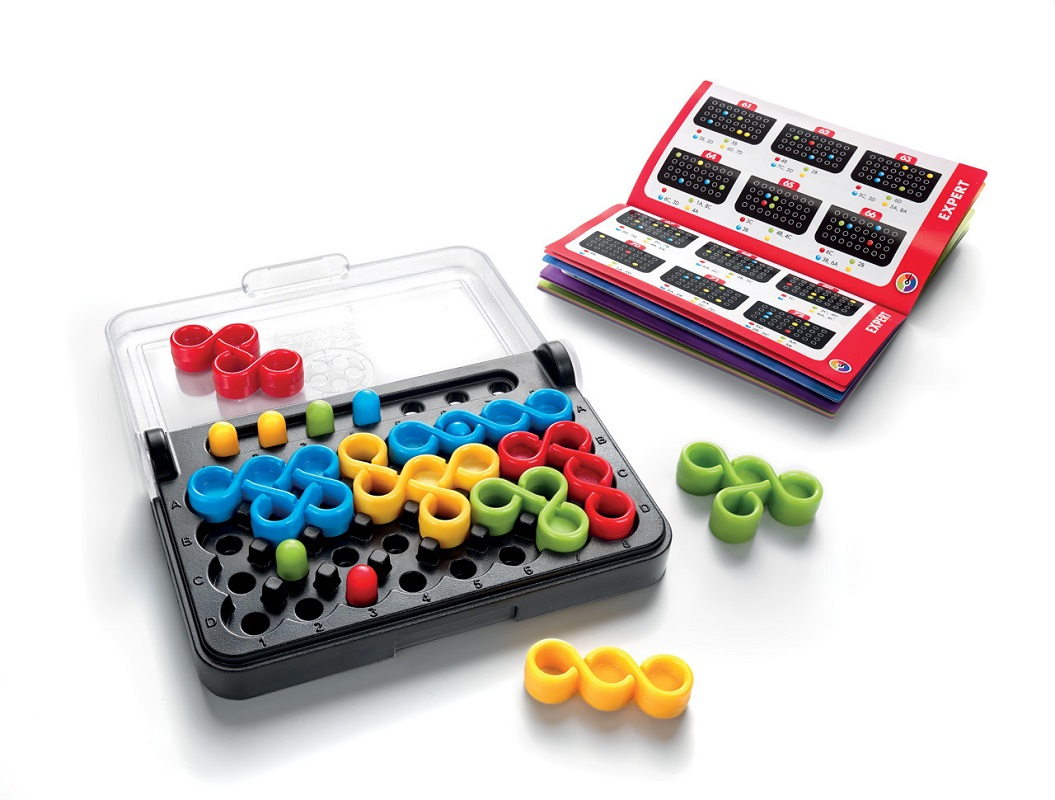
\includegraphics[width=0.5\textwidth]{figs/IQtwistintroduction.jpg}
    \caption{IQ Twist game, adopted from~\cite{r21}}
    \label{fig:IQ_twist_game}
\end{figure}
\subsection{Variables}
Above all, the initial state of each piece is defined in Figure~\ref{fig:allinit}.
\begin{figure}[htbp]
\begin{subfigure}[b]{.24\textwidth}
\centering

\includegraphics[width=0.75\textwidth]{figs/yellow1.jpg}
\caption{Initial state of yellow1}
  \label{fig:2Dyellow1}
\end{subfigure}
\begin{subfigure}[b]{.24\textwidth}
\centering
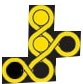
\includegraphics[width=0.75\textwidth]{figs/yellow2.jpg}
\caption{Initial state of yellow2}
  \label{fig:2Dyellow2}
\end{subfigure}
\begin{subfigure}[b]{.24\textwidth}
\centering
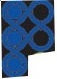
\includegraphics[width =0.5\textwidth]{figs/blue1.jpg}
\caption{Initial state of blue1}
  \label{fig:2Dblue1}
\end{subfigure}
\begin{subfigure}[b]{.24\textwidth}
\centering

\includegraphics[width=\textwidth]{figs/blue2.jpg}
\caption{Initial state of blue2}
  \label{fig:2Dblue2}
\end{subfigure}
\begin{subfigure}[b]{.24\textwidth}
\centering

\includegraphics[width=0.75\textwidth]{figs/green1.jpg}
\caption{Initial state of green1}
  \label{fig:2Dgreen1}
\end{subfigure}
\begin{subfigure}[b]{.24\textwidth}
\centering

\includegraphics[width =0.5\textwidth]{figs/green2.jpg}
\caption{Initial state of green2}
  \label{fig:2Dgreen2}
\end{subfigure}
\begin{subfigure}[b]{.24\textwidth}
\centering

\includegraphics[width =\textwidth]{figs/red1.jpg}
\caption{Initial state of red1}
  \label{fig:2Dred1}
\end{subfigure}
\begin{subfigure}[b]{.24\textwidth}
\centering

\includegraphics[width=0.75\textwidth]{figs/red2.jpg}
\caption{Initial state of red2}
  \label{fig:2Dred2}
\end{subfigure}
\caption{Initial state of each piece}
  \label{fig:allinit}
\end{figure}
For this model, there are some rules. Firstly, all the variables are corresponding to the specific units. As an example, for piece yellow2, Figure~\ref{fig:namerules} shows that the $V_{y21}$ is used to represent the left and bottom unit. For other variables, we name them as $V_{y22}$, $V_{y23}$, $V_{y24}$ and $V_{y25}$, which follows the order from left to right and bottom-up. In addition, there are 7 pegs. Therefore, the variables can be represented as \VUnits and \VPegs,
\begin{equation}
\begin{aligned}
\VUnits=\{&V_{y11},V_{y12},V_{y13},\\&V_{y21},V_{y22},V_{y23},V_{y24},V_{y25},\\&V_{b11},V_{b12},V_{b13},V_{b14},
V_{b15},\\&V_{b21},V_{b22},V_{b23},V_{b24},\\&V_{g11},V_{g12},V_{g13},V_{g14},\\&V_{g21},V_{g22},V_{g23},\\&V_{r11},
V_{r12},V_{r13},V_{r14},\\&V_{r21},V_{r22},V_{r23},V_{r24}\},\\
\\\VPegs = \{&V_{py1}, V_{py2}, V_{pb1}, V_{pb2}, V_{pg1}, V_{pg2}, V_{pr}\},\\
\\V = &\VUnits \cup \VPegs.
\end{aligned}
\end{equation}
\begin{figure}[htbp]
    \centering
    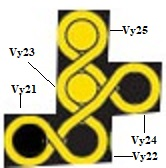
\includegraphics[width=0.3\textwidth]{figs/example.jpg}
    \caption{Name rules for yellow2}
    \label{fig:namerules}
\end{figure}
\subsection{Domains}
\begin{figure}[htbp]
\centering
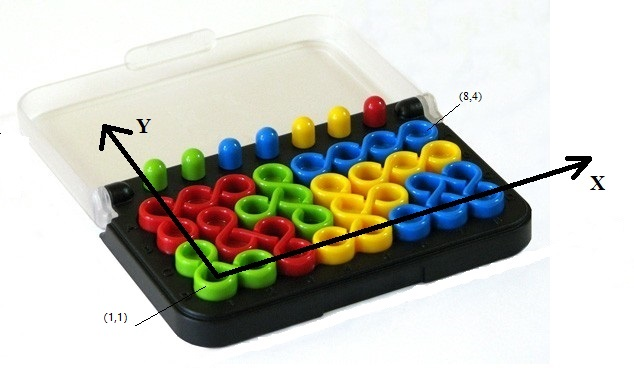
\includegraphics[width=0.8\textwidth]{figs/IQtwistboard.jpg}
\caption{The coordinate system for IQ Twist, revised from~\cite{r22}}
    \label{fig:coordinate}
\end{figure}
For the board, Figure~\ref{fig:coordinate} shows that the 2D coordinate system is used to represent the positions. In our model, all positions are represented as tuples and the elements in the tuples are int. In addition, each tuple contains 2 int. The left and bottom position as $(1,1)$ and the right and top as $(8,4)$. So, all placements will be between them. Considering a position $(x_{0},y_{0})$, we get
\begin{equation}
\begin{aligned}
&0<x_{0} \leq 8,\\
&0<y_{0} \leq 4.
\end{aligned}
\end{equation}
The placements for each unit of pieces must on the board, therefore, we get
\begin{equation}
\forall  v \in \VUnits \hspace{1ex},\hspace{1ex} D(v)=\{(i,j) \in \mathbb{Z} \times \mathbb{Z}	\mid  0<i \leq 8 \hspace{1ex} , \hspace{1ex} 0<j \leq 4\}.\\
\end{equation}
The pegs are special because they can be put in any places on the board or not on the board. So, the domain of pegs is
\begin{equation}
\forall  v \in \VPegs \hspace{1ex},\hspace{1ex} D(v)=\{(0,0)\} \hspace{1ex} \cup \hspace{1ex}\{(i,j) \in \mathbb{Z} \times \mathbb{Z}\mid  0<i \leq 8 \hspace{1ex} , \hspace{1ex} 0<j \leq 4\}.
\end{equation}
\subsection{2D Rotation Matrix}
\label{section:2Drotationmatrix}
To clarify how to obtain all configurations for each piece. I'd like to introduce 2D rotation matrix. 
\\In Figure~\ref{fig:explanation2D}, the unit which is corresponding to the first variable $V_{y21}$ will be considered as a point $(x_{0},y_{0})$. If we assign (0,0) to $(x_{0},y_{0})$, the $V_{y21}$, $V_{y22}$, $V_{y23}$, $V_{y24}$ and $V_{y25}$ can be respectively represented as $(0,0)$, $(1,0)$, $(1,1)$, $(2,1)$ and $(1,2)$, which indicate that all other variables are connection with the first variables. For example, there are relationships
\begin{equation}
\begin{aligned}
&x_{V_{y21}}+1=x_{V_{y22}},\\
&y_{V_{y21}}=y_{V_{y22}},
\end{aligned}
\end{equation}
between $V_{y21}$ and $V_{y22}$.
\begin{figure}[htbp]
\centering
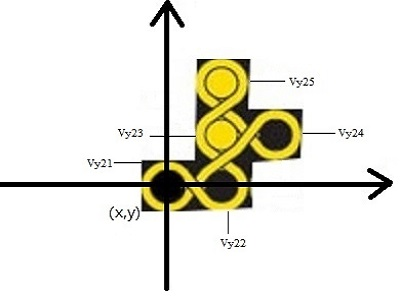
\includegraphics[width=0.5\textwidth]{figs/explanation2D.jpg}
\caption{The explanation of 2D rotation}
    \label{fig:explanation2D}
\end{figure}
Therefore, all other placements can be obtained from the initial state of the piece by rotations around the unit of piece $V_{y21}$.\\
Tobias and Krantz \cite{r9} mention that 2D rotation by an angle $\theta$ around the origin of coordinate can be described as a matrix
\begin{equation}
R(\theta)=\begin{bmatrix}
\cos\theta & -\sin\theta\\
\sin\theta & \cos\theta\\
\end{bmatrix}.
\end{equation}
If the initial position is (x,y), we can get the position after the rotation by
\begin{equation}
\label{equation:rotation}
\begin{bmatrix}
x'\\
y'\\
\end{bmatrix}
=\begin{bmatrix}
\cos\theta & -\sin\theta\\
\sin\theta & \cos\theta\\
\end{bmatrix}
\begin{bmatrix}
x\\
y\\
\end{bmatrix},
\end{equation}
which implies that 
\begin{equation}
\label{equation:formula1}
\begin{aligned}
&x'=x\cos\theta-y\sin\theta,\\
&y'=x\sin\theta+y\cos\theta.
\end{aligned}
\end{equation}
Therefore, if we assign 0, 90, 180 and 270 degrees to $\theta$, we get four configurations:
\begin{itemize}
  \item $x'=x\cos0^{\circ} - y\sin0^{\circ}\hspace{20pt},y'=x\sin0^{\circ} + y\cos0^{\circ}\hspace{24pt}\implies x'=x\hspace{10pt}, y'=y$
  \item $x'=x\cos90^{\circ} - y\sin90^{\circ}\hspace{10pt},y'=x\sin90^{\circ} + y\cos90^{\circ}\hspace{12pt}\implies x'=-y, y'=x$
  \item $x'=x\cos180^{\circ} - y\sin180^{\circ}, y'=x\sin180^{\circ} + y\cos180^{\circ} \implies x'=-x, y'=-y$
  \item $x'=x\cos270^{\circ} - y\sin270^{\circ}, y'=x\sin270^{\circ} + y\cos270^{\circ} \implies x'=y\hspace{10pt},y'=-x$
  \label{rotation4}
\end{itemize}
In IQ Twist, there exists a mirroring operation which corresponds to flpping a piece, if a unit of piece flip over around the y-axis, we get  (-x,y) from (x,y). Similarly, all the four configurations flip over around the y-axis. We get four more configurations: 
\begin{itemize}
  \item  $x'=x\hspace{10pt}, y'=y\hspace{10pt}$    flip over around the y-axis $\implies x''=-x\hspace{8pt},y''=y$
  \item  $x'=-y, y'=x\hspace{10pt}$                flip over around the y-axis $\implies x''=y,y''=x$
  \item  $x'=-x, y'=-y$               flip over around the y-axis $\implies x''=x, y''=-y$
  \item  $x'=y\hspace{10pt},y'=-x$    flip over around the y-axis $\implies x''=-y\hspace{8pt}, y''=-x$
  \label{mirrorrotate4}
\end{itemize}
Therefore, there should be a total of eight configurations for each unit of pieces. Similarly, for all units of piece in Figure~\ref{fig:explanation2D}, if we assign $(0,0)$ to $(x_{0},y_{0})$, the process of rotation for each other unit of the piece can be represented by Equation~\ref{equation:rotation}. Accordingly, we get eight possible configurations
\begin{itemize}
 \item $V_{y21}=(0,0)$, $V_{y22}=(1,0)$, $V_{y23}=(1,1)$, $V_{y24}=(2,1)$, $V_{y25}=(1,2)$,
 \item $V_{y21}=(0,0)$, $V_{y22}=(0,1)$, $V_{y23}=(-1,1)$, $V_{y24}=(-1,2)$, $V_{y25}=(-2,1)$,
 \item $V_{y21}=(0,0)$, $V_{y22}=(-1,0)$, $V_{y23}=(-1,-1)$, $V_{y24}=(-2,-1)$, $V_{y25}=(-1,-2)$,
 \item $V_{y21}=(0,0)$, $V_{y22}=(0,-1)$, $V_{y23}=(1,-1)$, $V_{y24}=(1,-2)$, $V_{y25}=(2,-1)$,
 \item $V_{y21}=(0,0)$, $V_{y22}=(-1,0)$, $V_{y23}=(-1,1)$, $V_{y24}=(-2,1)$, $V_{y25}=(-1,2)$,
 \item $V_{y21}=(0,0)$, $V_{y22}=(0,1)$, $V_{y23}=(1,1)$, $V_{y24}=(1,2)$, $V_{y25}=(2,1)$,
 \item $V_{y21}=(0,0)$, $V_{y22}=(1,0)$, $V_{y23}=(1,-1)$, $V_{y24}=(2,-1)$, $V_{y25}=(1,-2)$,
 \item $V_{y21}=(0,0)$, $V_{y22}=(-1,0)$, $V_{y23}=(-1,-1)$, $V_{y24}=(-2,-1)$, $V_{y25}=(-1,-2)$.
\end{itemize}
In our case, the piece can be moved as long as all units of piece on the board. Both the $x_{0}$ and $y_{0}$ can be variables, hence, we get the general forms
\begin{itemize}
 \item $V_{y21}=(x_{0},y_{0})$, $V_{y22}=(x_{0}+1,y_{0})$, $V_{y23}=(x_{0}+1,y_{0}+1)$, $V_{y24}=(x_{0}+2,y_{0}+1)$, $V_{y25}=(x_{0}+1,y_{0}+2)$,
 \item $V_{y21}=(x_{0},y_{0})$, $V_{y22}=(x_{0},y_{0}+1)$, $V_{y23}=(x_{0}-1,y_{0}+1)$, $V_{y24}=(x_{0}-1,y_{0}+2)$, $V_{y25}=(x_{0}-2,y_{0}+1)$,
 \item $V_{y21}=(x_{0},y_{0})$, $V_{y22}=(x_{0}-1,y_{0})$, $V_{y23}=(x_{0}-1,y_{0}-1)$, $V_{y24}=(x_{0}-2,y_{0}-1)$, $V_{y25}=(x_{0}-1,y_{0}-2)$,
 \item $V_{y21}=(x_{0},y_{0})$, $V_{y22}=(x_{0},y_{0}-1)$, $V_{y23}=(x_{0}+1,y_{0}-1)$, $V_{y24}=(x_{0}+1,y_{0}-2)$, $V_{y25}=(x_{0}+2,y_{0}-1)$,
 \item $V_{y21}=(x_{0},y_{0})$, $V_{y22}=(x_{0}-1,y_{0})$, $V_{y23}=(x_{0}-1,y_{0}+1)$, $V_{y24}=(x_{0}-2,y_{0}+1)$, $V_{y25}=(x_{0}-1,y_{0}+2)$,
 \item $V_{y21}=(x_{0},y_{0})$, $V_{y22}=(x_{0},y_{0}+1)$, $V_{y23}=(x_{0}+1,y_{0}+1)$, $V_{y24}=(x_{0}+1,y_{0}+2)$, $V_{y25}=(x_{0}+2,y_{0}+1)$,
 \item $V_{y21}=(x_{0},y_{0})$, $V_{y22}=(x_{0}+1,y_{0})$, $V_{y23}=(x_{0}+1,y_{0}-1)$, $V_{y24}=(x_{0}+2,y_{0}-1)$, $V_{y25}=(x_{0}+1,y_{0}-2)$,
 \item $V_{y21}=(x_{0},y_{0})$, $V_{y22}=(x_{0}-1,y_{0})$, $V_{y23}=(x_{0}-1,y_{0}-1)$, $V_{y24}=(x_{0}-2,y_{0}-1)$, $V_{y25}=(x_{0}-1,y_{0}-2)$.
\end{itemize}
\subsection{Constrains}
Firstly, there should be no 2 different unit variables contain the same value
\begin{equation}
\begin{aligned}
&\forall V_{m},V_{n} \in \VUnits,V_{m} \neq V_{n},\\
&\Constraints{m}{n}=\{((x_{1},y_{1}),(x_{2},y_{2}))\in \Domain{m} \times \Domain{n}\mid x_{1} \neq x_{2}   \hspace{1ex} or \hspace{1ex}  y_{1} \neq y_{2}\}.
\end{aligned}
\end{equation}
Similarly, there should be no 2 different reg variables contain the same value except both of them are not on the board
\begin{equation}
\begin{aligned}
&\forall V_{m},V_{n}\in \VPegs, V_{m} \neq V_{n},\\
&\Constraints{m}{n}=\{((x_{1},y_{1}),(x_{2},y_{2}))\in \Domain{m}\times \Domain{n}\mid x_{1} \neq x_{2}   \hspace{1ex} or \hspace{1ex}  y_{1} \neq y_{2}\}\hspace{1pt}\cup \\
&\{((0,0),(0,0))\}.
\end{aligned}
\end{equation}
As is mentioned in Chapter~\ref{section:2Drotationmatrix}, there should be eight configurations for general pieces. Figure~\ref{fig:Exampleof8} shows the eight configurations for yellow2. Hence,
\begin{figure}[htbp]
\centering
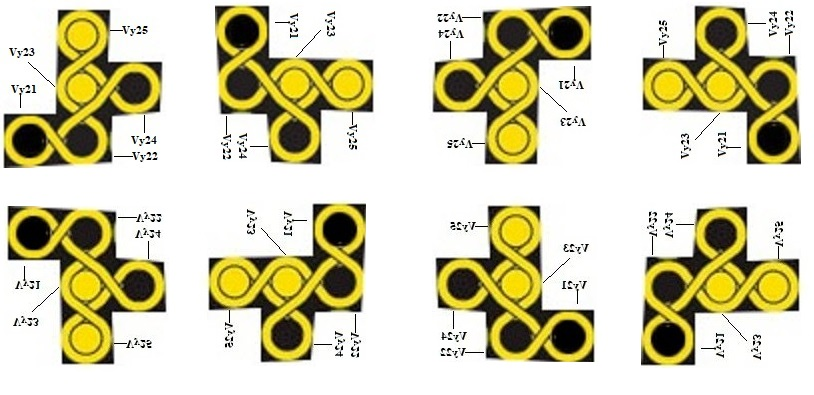
\includegraphics[width =\textwidth]{figs/domainexplain.jpg}
    \caption{Example of 8 configurations}
    \label{fig:Exampleof8}
\end{figure}
\begin{equation}
\begin{aligned}
\Cons{y21}{y22}{y23}{y24}{y25}=\{&((x_{1},y_{1}),(x_{2},y_{2}),(x_{3},y_{3}),(x_{4},y_{4}),(x_{5},y_{5}))\in \\
&\Domain {y21} \times \Domain{y22}\times \Domain{y23}\times \Domain{y24}\times \Domain{y25} \mid\\
&(x_{2} = x_{1} + 1,\hspace{1ex}y_{2} = y_{1},\hspace{1ex}x_{3} = x_{1}+1,\hspace{1ex}y_{3} = y_{1}+1,
\\&x_{4} = x_{1}+2,\hspace{1ex}y_{4} = y_{1}+1,\hspace{1ex}x_{5} = x_{1}+1,\hspace{1ex}y_{5} = y_{1}+2)\hspace{1ex} or \\
&(x_{2} = x_{1} ,\hspace{1ex}y_{2} = y_{1}+1,\hspace{1ex}x_{3} = x_{1}-1,\hspace{1ex}y_{3} = y_{1}+1,
\\&x_{4} = x_{1}-1,\hspace{1ex}y_{4} = y_{1}+2,\hspace{1ex}x_{5} = x_{1}-2,\hspace{1ex}y_{5} = y_{1}+1)\hspace{1ex} or \\
&(x_{2} = x_{1}-1 ,\hspace{1ex}y_{2} = y_{1},\hspace{1ex}x_{3} = x_{1}-1,\hspace{1ex}y_{3} = y_{1}-1,
\\&x_{4} = x_{1}-2,\hspace{1ex}y_{4} = y_{1}-1,\hspace{1ex}x_{5} = x_{1}-1,\hspace{1ex}y_{5} = y_{1}-2)\hspace{1ex} or \\
&(x_{2} = x_{1} ,\hspace{1ex}y_{2} = y_{1}-1,\hspace{1ex}x_{3} = x_{1}+1,\hspace{1ex}y_{3} = y_{1}-1,
\\&x_{4} = x_{1}+1,\hspace{1ex}y_{4} = y_{1}-2,\hspace{1ex}x_{5} = x_{1}+2,\hspace{1ex}y_{5} = y_{1}-1)\hspace{1ex} or \\
&(x_{2} = x_{1}-1 ,\hspace{1ex}y_{2} = y_{1},\hspace{1ex}x_{3} = x_{1}-1,\hspace{1ex}y_{3} = y_{1}+1,
\\&x_{4} = x_{1}-2,\hspace{1ex}y_{4} = y_{1}+1,\hspace{1ex}x_{5} = x_{1}-1,\hspace{1ex}y_{5} = y_{1}+2)\hspace{1ex} or \\
&(x_{2} = x_{1} ,\hspace{1ex}y_{2} = y_{1}-1,\hspace{1ex}x_{3} = x_{1}-1,\hspace{1ex}y_{3} = y_{1}-1,
\\&x_{4} = x_{1}-1,\hspace{1ex}y_{4} = y_{1}-2,\hspace{1ex}x_{5} = x_{1}-2,\hspace{1ex}y_{5} = y_{1}-1)\hspace{1ex} or \\
&(x_{2} = x_{1}+1 ,\hspace{1ex}y_{2} = y_{1},\hspace{1ex}x_{3} = x_{1}+1,\hspace{1ex}y_{3} = y_{1}-1,
\\&x_{4} = x_{1}+2,\hspace{1ex}y_{4} = y_{1}-1,\hspace{1ex}x_{5} = x_{1}+1,\hspace{1ex}y_{5} = y_{1}-2)\hspace{1ex} or \\
&(x_{2} = x_{1} ,\hspace{1ex}y_{2} = y_{1}+1,\hspace{1ex}x_{3} = x_{1}+1,\hspace{1ex}y_{3} = y_{1}+1,
\\&x_{4} = x_{1}+1,\hspace{1ex}y_{4} = y_{1}+2,\hspace{1ex}x_{5} = x_{1}+2,\hspace{1ex}y_{5} = y_{1}+1)\hspace{3ex}\}.
\end{aligned}
\end{equation}
Similarly, every piece can get the similar constraints (Appendix~\ref{appendix:2Dpieces}). Furthermore, for the pegs, unless they are not on the board, there must be a hollow unit of pieces which contains the same color with the pegs to match them. As an instance, for yellow peg1, there are 4 hollow units of yellow pieces. Therefore, we can obtain
\begin{equation}
\begin{aligned}  
\Constraint{py1} = &\{((x_{1},y_{1}),(x_{2},y_{2}))\in \Domain{py1} \times \Domain{y11}\mid x_{2} = x_{1} \hspace{1ex} , \hspace{1ex}  y_{2} = y_{1}\}\hspace{1ex} \cup  
\\&\{((x_{1},y_{1}),(x_{2},y_{2}))\in \Domain{py1} \times \Domain{y21}\mid x_{2} = x_{1} \hspace{1ex} , \hspace{1ex}  y_{2} = y_{1}\}\hspace{1ex} \cup 
\\&\{ ((x_{1},y_{1}),(x_{2},y_{2}))\in \Domain{py1} \times \Domain{y22}\mid x_{2} = x_{1} \hspace{1ex} , \hspace{1ex}  y_{2} = y_{1}\}\hspace{1ex}\cup 
\\& \{((x_{1},y_{1}),(x_{2},y_{2}))\in \Domain{py1} \times \Domain{y24}\mid x_{2} = x_{1} \hspace{1ex} , \hspace{1ex}  y_{2} = y_{1}\} \hspace{1ex}\cup
\\& \{(0,0)\}.
\end{aligned}
\end{equation}
Accordingly, every peg can get the similar constraints (Appendix~\ref{appendix:2Dpegs}).
\label{section:implementation1}
\section{ZIG ZAG Puzzler}
Zig Zag Puzzler is a 3D puzzle game with 2 playing modes. Both games aim to place all pieces to full fill the game boards. In addition, for both of them, there are some pieces placed in advance to set the difficulty (Figure~\ref{fig:ZIG_ZAG_Puzzler_playing_modes}). Generally, the fewer pieces are placed in advance, the more difficult to solve the puzzler.
\begin{figure}[htbp]
    \centering
    \begin{subfigure}[b]{0.4\textwidth}
    
\includegraphics[width=\textwidth]{figs/zig_zag_mode1.jpg}
    \caption{One example of ZIG ZAG Puzzler playing mode1}
    \end{subfigure}
    \begin{subfigure}[b]{0.4\textwidth}
    
\includegraphics[width=\textwidth]{figs/zig_zag_mode2.jpg}
    \caption{One example of ZIG ZAG Puzzler playing mode2}
    \end{subfigure}
    \caption{ZIG ZAG Puzzler examples, adopted from~\cite{r23}}
    \label{fig:ZIG_ZAG_Puzzler_playing_modes}
\end{figure}
\\In this part, the designs of CSP models for Zig Zag Puzzler will be discussed. Generally, there are 2 playing modes, which uses the same pieces but different boards. On the condition of the two coordinates based on the same system which means both of them adopt right-handed coordinate or left-handed coordinate (Figure~\ref{figure:Cartesiancoordinate}), both of them can adopt the same variables and the same constraints but different domains. In our case, we adopt right-handed coordinate. 
\begin{figure}[htbp]
    \centering
    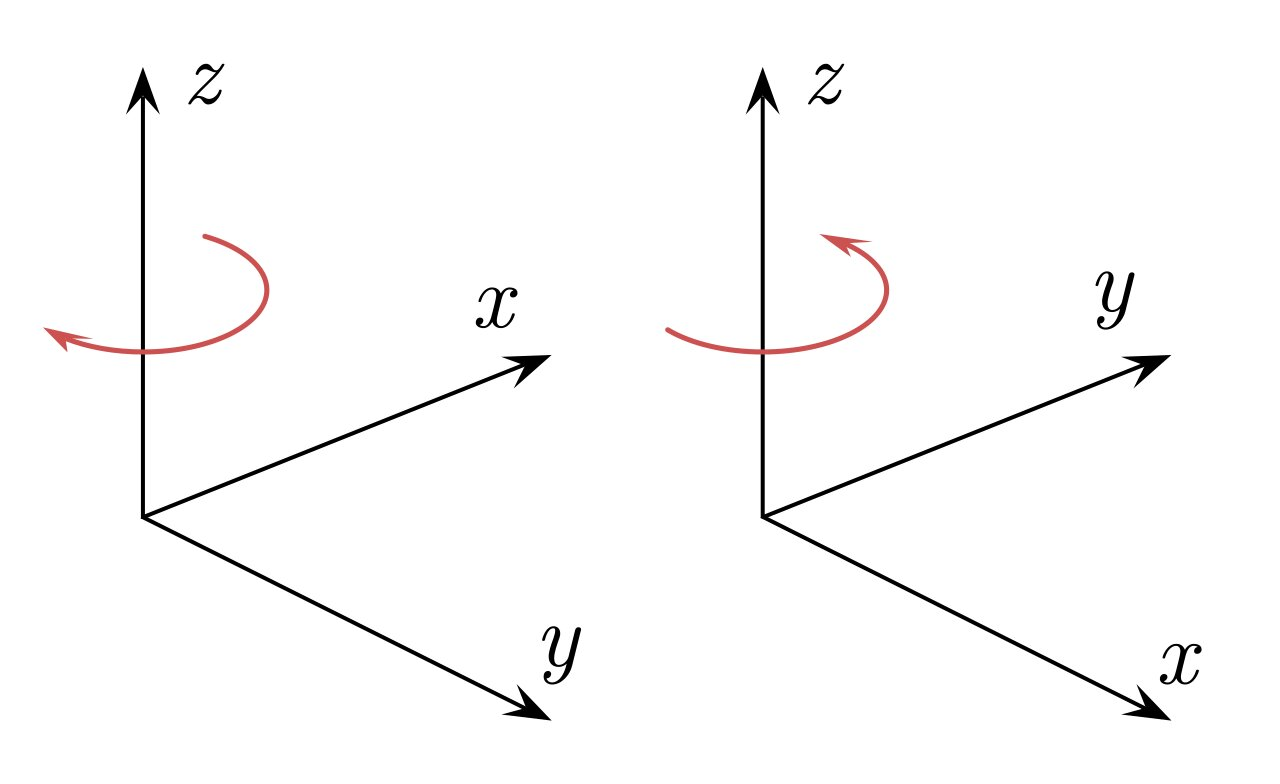
\includegraphics[width=0.8\textwidth]{figs/Cartesian_coordinate_system_handedness}
    \caption{Left-handed (left) coordinate and right-handed coordinate (right), adopted from~\cite{r20}}
    \label{figure:Cartesiancoordinate}
\end{figure}
\subsection{Variables}
Firstly, the initial state of each piece is defined in Figure~\ref{fig:all3Dinit}.
\label{section:3Dgame}
\begin{figure}[htbp]
\centering
\begin{subfigure}[b]{0.25\textwidth}
\centering
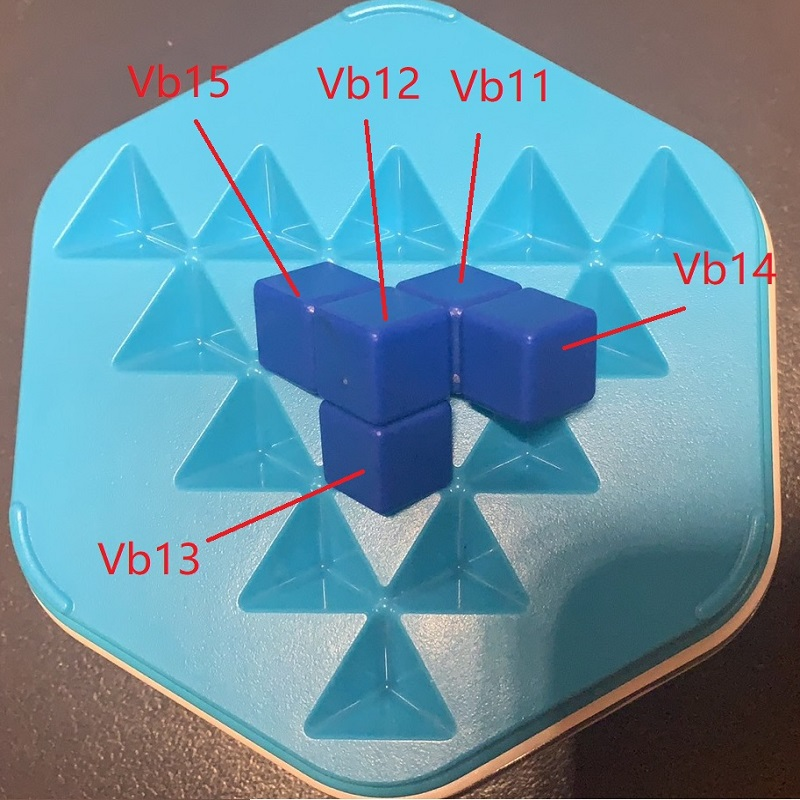
\includegraphics[width=\textwidth]{figs/3Dblue1.jpg}
\caption{The variable explanation of blue1}
  \label{fig:3Dblue1}
\end{subfigure}
\begin{subfigure}[b]{0.25\textwidth}
\centering
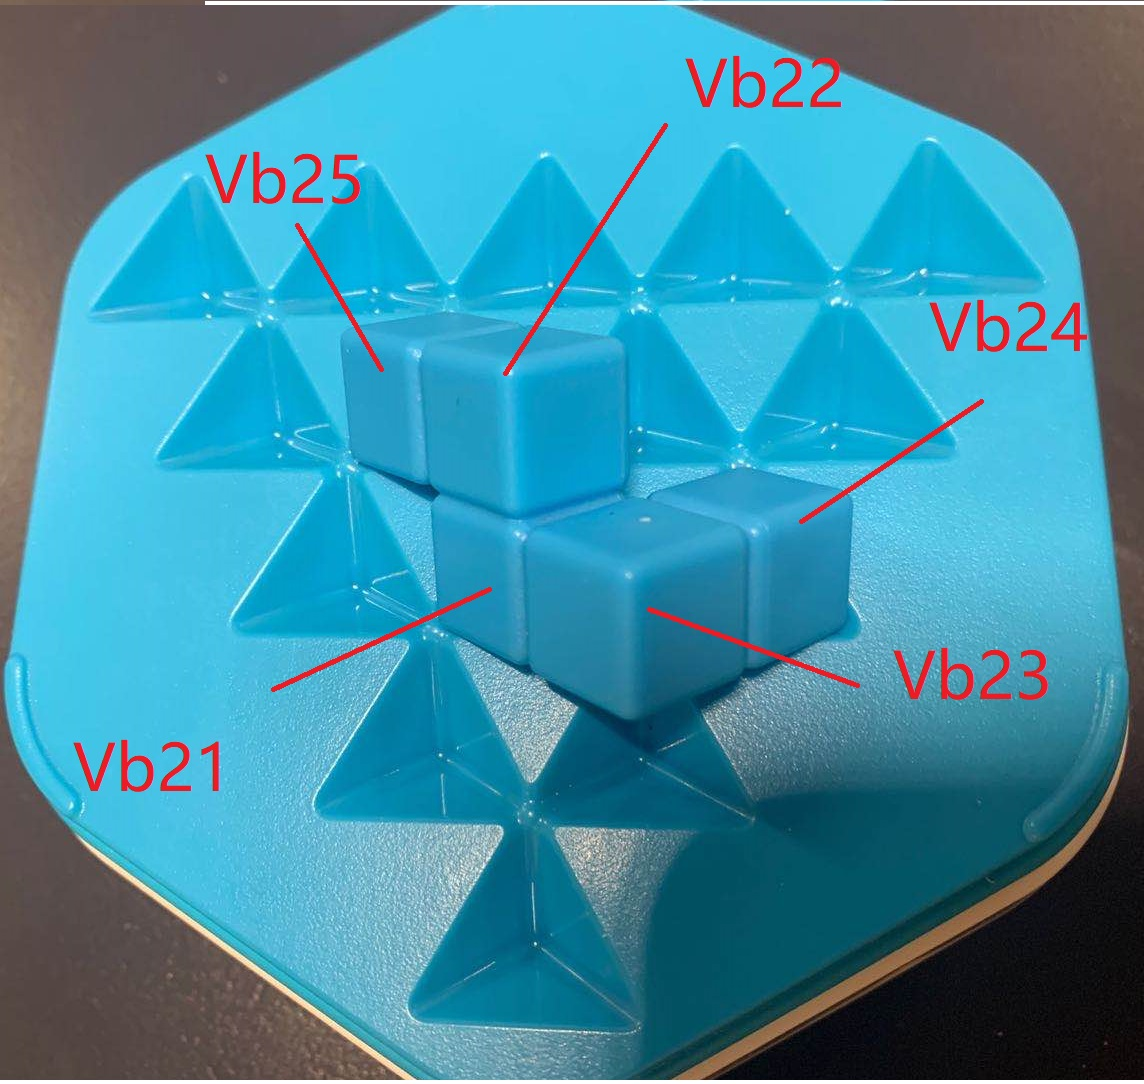
\includegraphics[width=\textwidth]{figs/3Dblue2.jpg}
\caption{The variable explanation of blue2}
  \label{fig:3Dblue2}
\end{subfigure}
\begin{subfigure}[b]{0.25\textwidth}
\centering
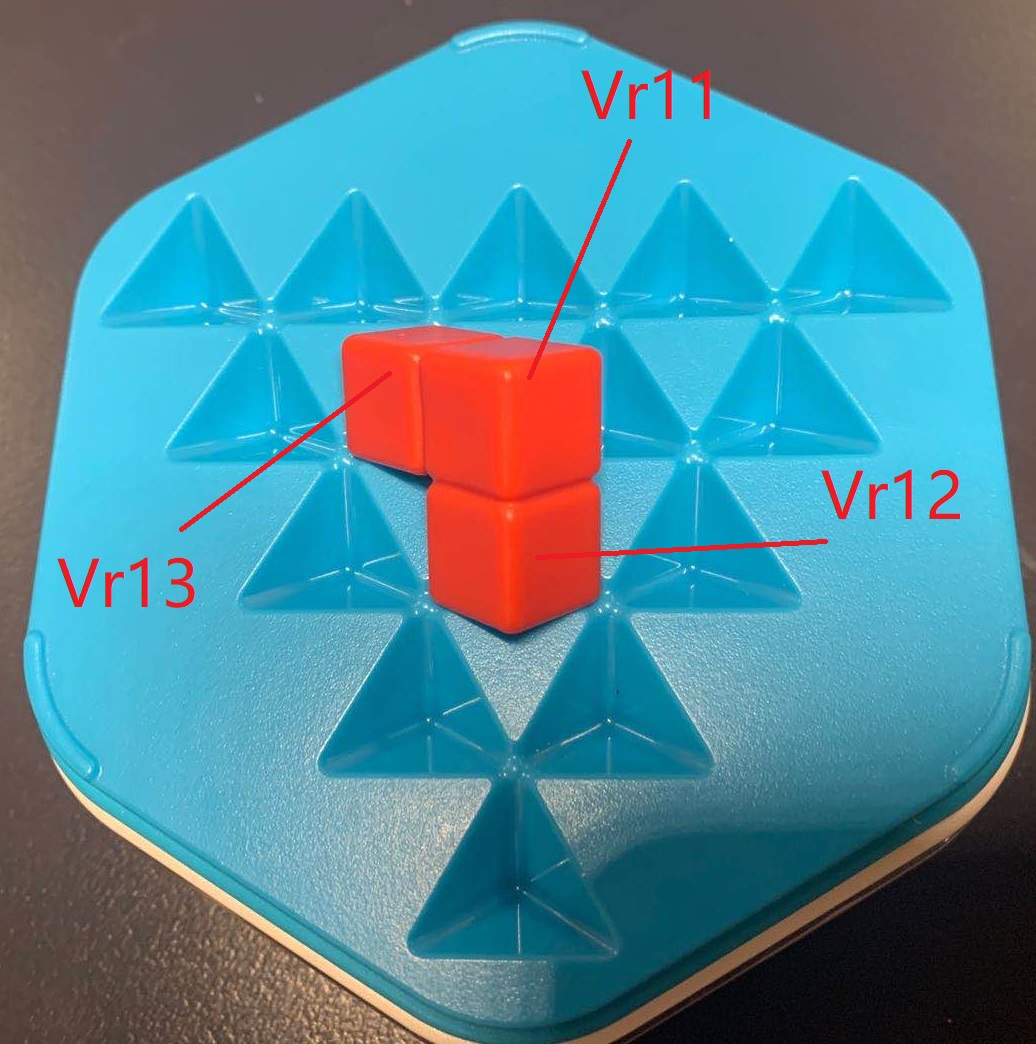
\includegraphics[width=\textwidth]{figs/3Dred1.jpg}
\caption{The variable explanation of red1}
  \label{fig:3Dred1}
\end{subfigure}
\begin{subfigure}[b]{0.25\textwidth}
\centering
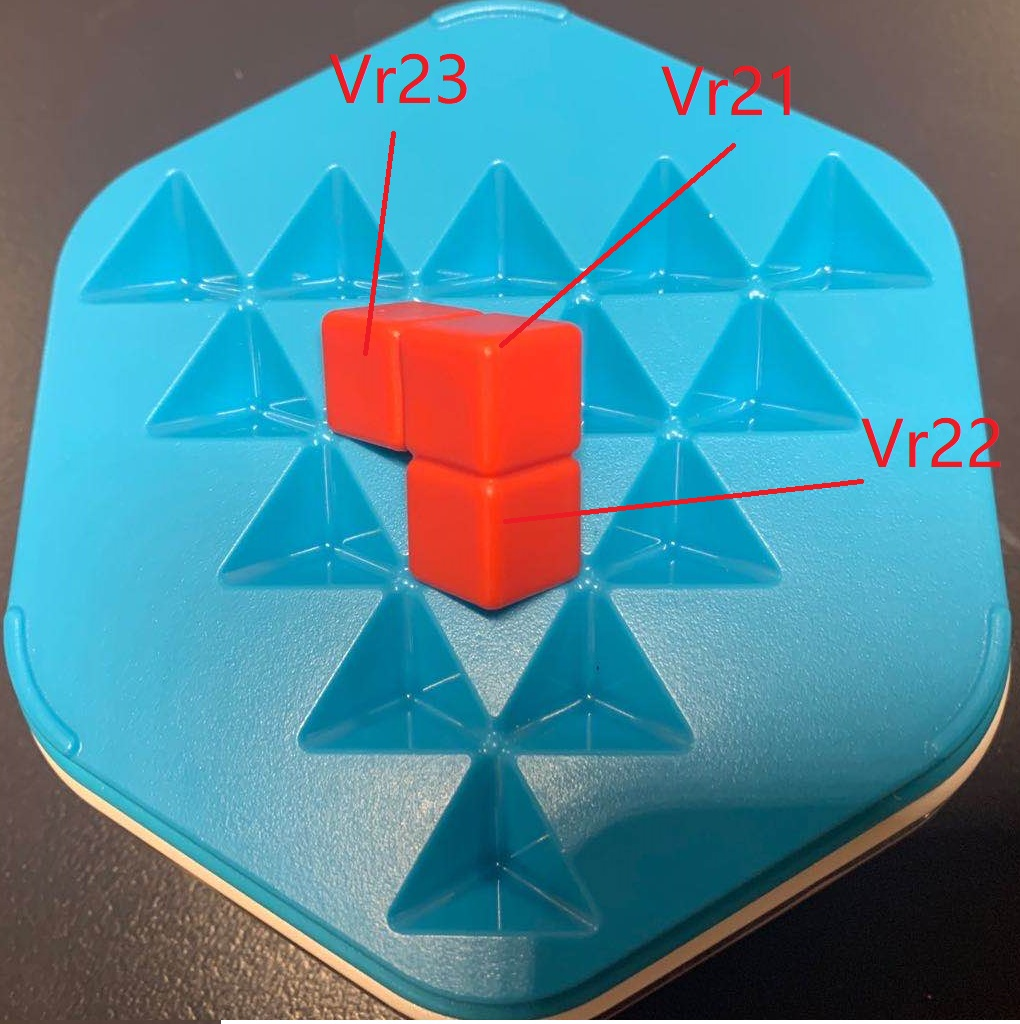
\includegraphics[width=\textwidth]{figs/3Dred2.jpg}
\caption{The variable explanation of red2}
  \label{fig:3Dred2}
\end{subfigure}
\begin{subfigure}[b]{0.25\textwidth}
\centering
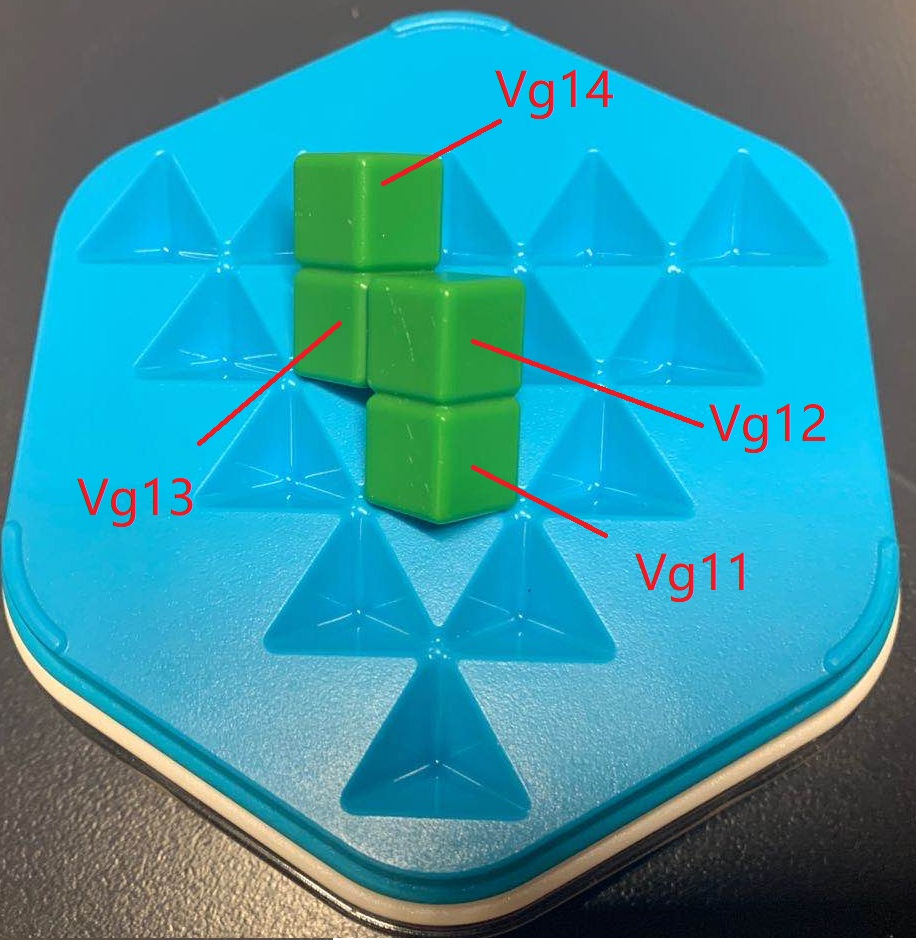
\includegraphics[width=\textwidth]{figs/3Dgreen1.jpg}
\caption{The variable explanation of green1}
  \label{fig:3Dgreen1}
\end{subfigure}
\begin{subfigure}[b]{0.25\textwidth}
\centering
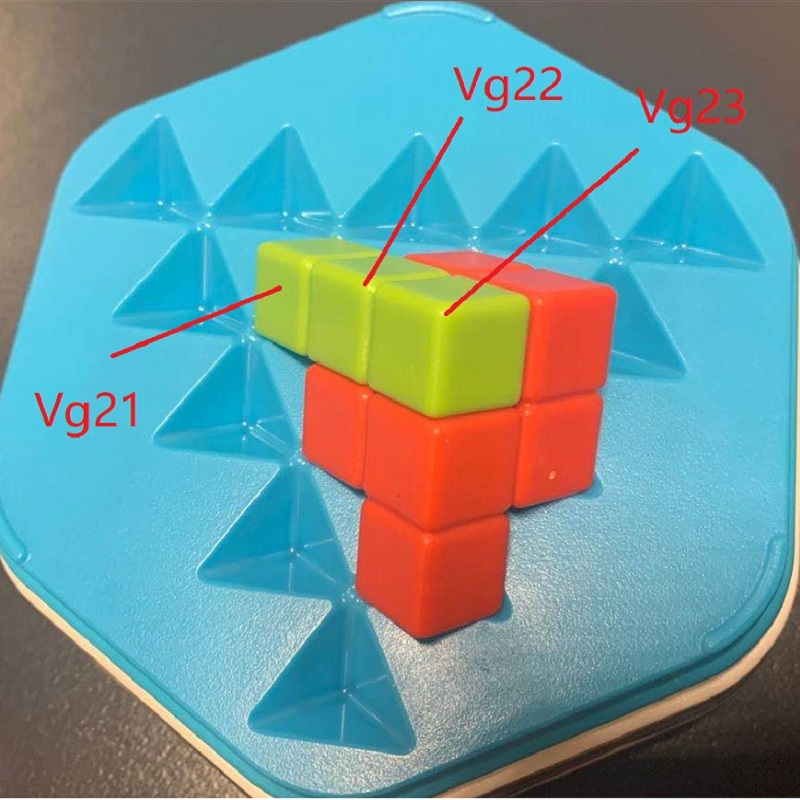
\includegraphics[width=\textwidth]{figs/3Dgreen2.jpg}
\caption{The variable explanation of green2}
  \label{fig:3Dgreen2}
\end{subfigure}
\begin{subfigure}[b]{0.25\textwidth}
\centering
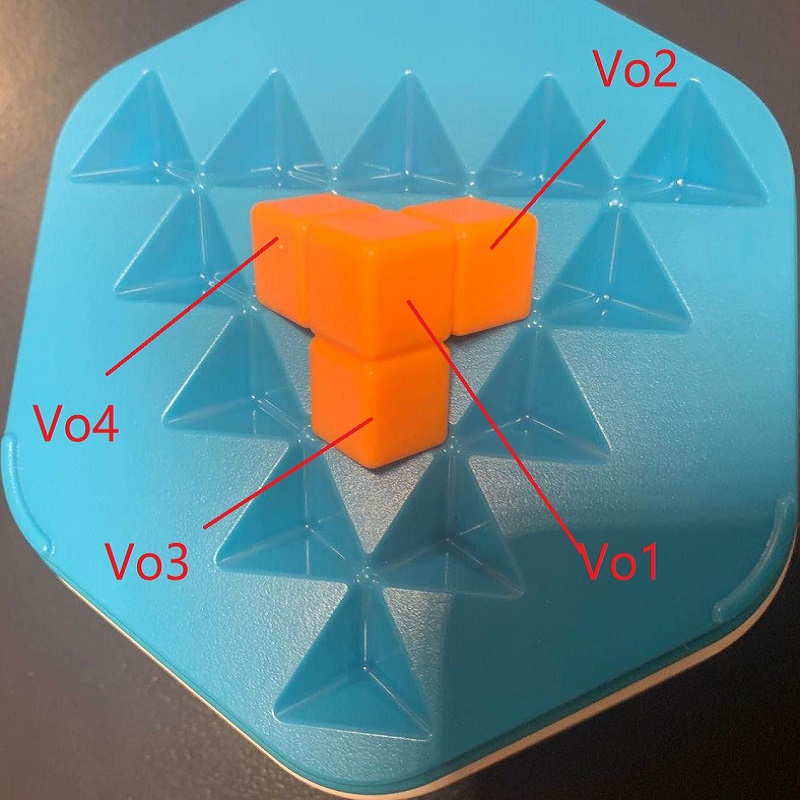
\includegraphics[width=\textwidth]{figs/3Dorange.jpg}
\caption{The variable explanation of orange}
  \label{fig:3Dorange}
\end{subfigure}
\begin{subfigure}[b]{0.25\textwidth}
\centering
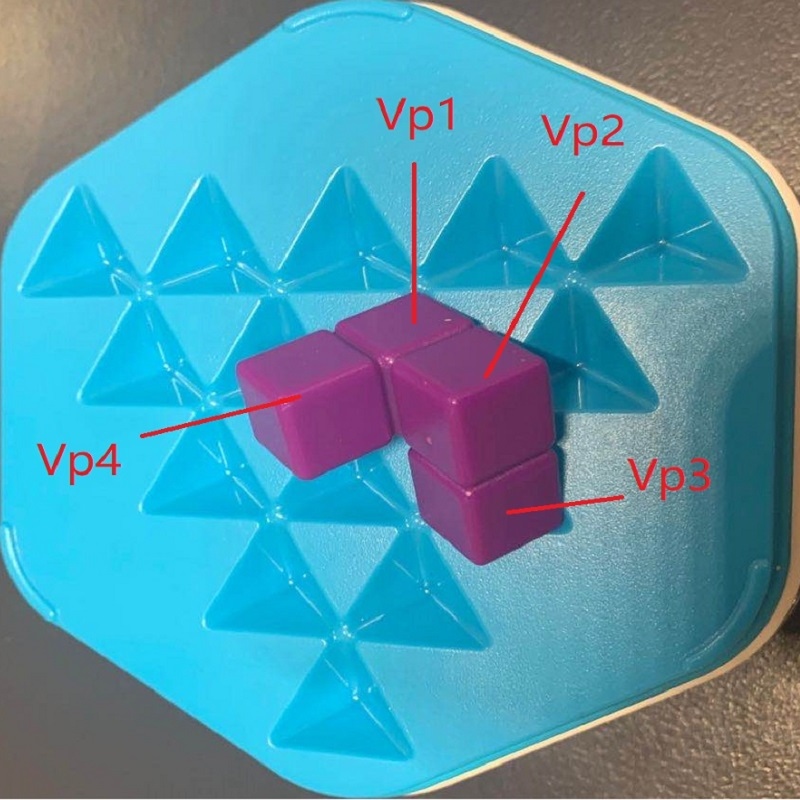
\includegraphics[width=\textwidth]{figs/3Dpurple.jpg}
\caption{The variable explanation of purple}
  \label{fig:3Dpurple}
\end{subfigure}
\begin{subfigure}[b]{0.25\textwidth}
\centering
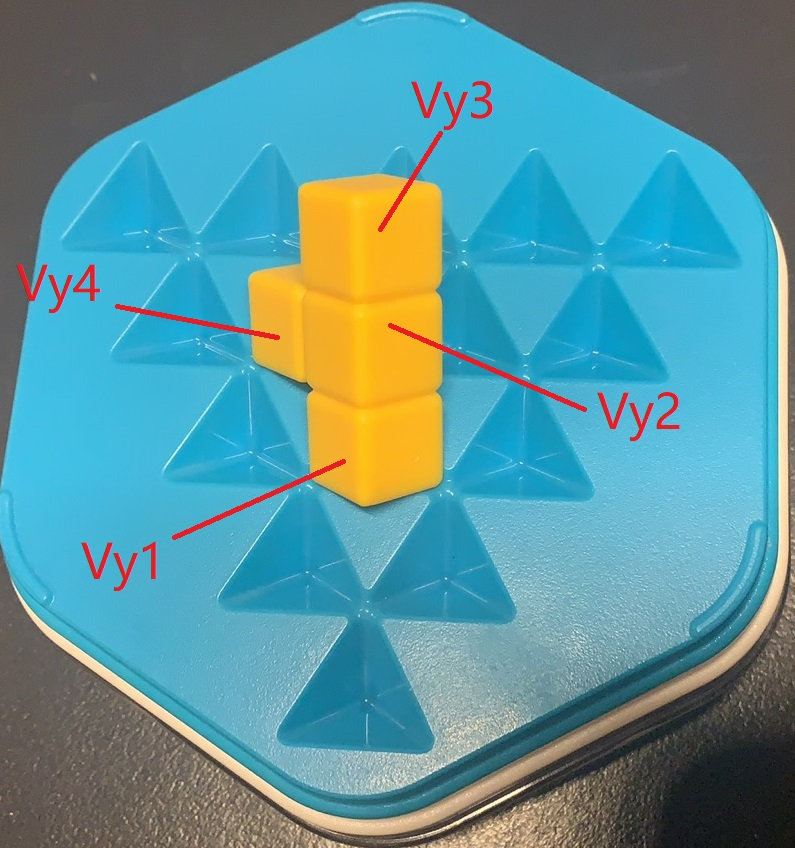
\includegraphics[width=\textwidth]{figs/3Dyellow.jpg}
\caption{The variable explanation of yellow}
  \label{fig:3Dyellow}
\end{subfigure}
\caption{Initial state of each piece}
  \label{fig:all3Dinit}
\end{figure}
It shows all the variables are corresponding to the specific units. Therefore, the variables can be defined as
\begin{equation}
\begin{aligned}
\VUnits=\{&V_{y1},V_{y2},V_{y3},V_{y4},\\&V_{b11},V_{b12},V_{b13},V_{b14},
V_{b15},\\&V_{b21},V_{b22},V_{b23},V_{b24},V_{b25},\\&V_{g11},V_{g12},V_{g13},V_{g14},\\&V_{g21},V_{g22},V_{g23},\\&V_{r11},
V_{r12},V_{r13},\\&V_{r21},V_{r22},V_{r23},\\&V_{o1},V_{o2},V_{o3},V_{o4},\\&V_{p1},V_{p2},V_{p3},V_{p4}\}.
\end{aligned}
\end{equation}
\subsection{Domains for Playing Mode 1 and 2}
\label{sec:3Ddomains}
Figure~\ref{fig:board1} and Figure~\ref{fig:board2} show how to create the coordinates for both modes to represent the positions of the boards. For of them, similar to IQ Twist, the positions are represented as tuples and the elements in tuples are int. But each tuple will contain 3 int. The unit of piece which is located in the origin of coordinate can be represented as $(1,1,1)$. So Considering one position $(x_{0},y_{0},z_{0})$.
\begin{figure}[htbp]
\centering
\begin{subfigure}[b]{.3\textwidth}
\centering
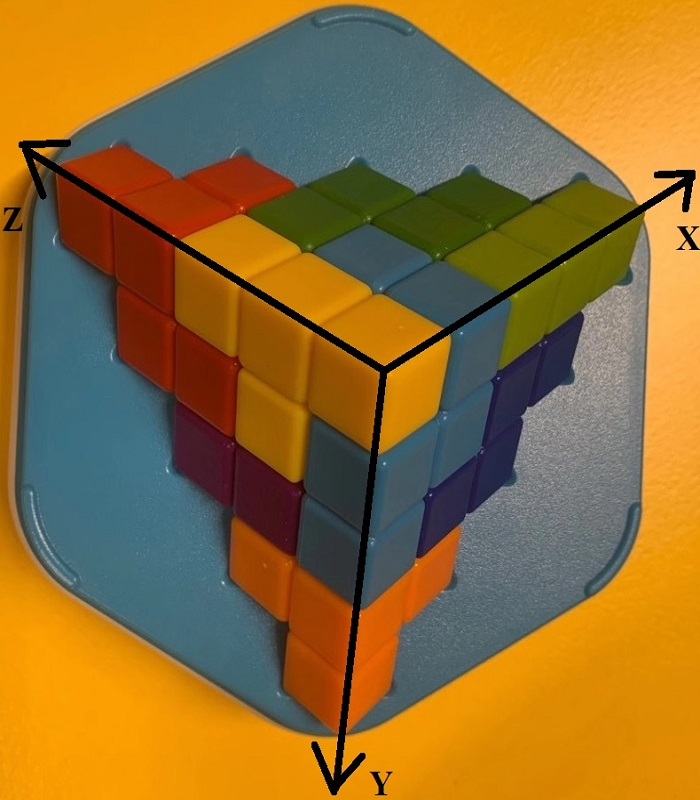
\includegraphics[width=\textwidth]{figs/ZIGZAGmodel1board.jpg}
\caption{}
\label{figure:mode1A}
\end{subfigure}
\begin{subfigure}[b]{.3\textwidth}
\centering
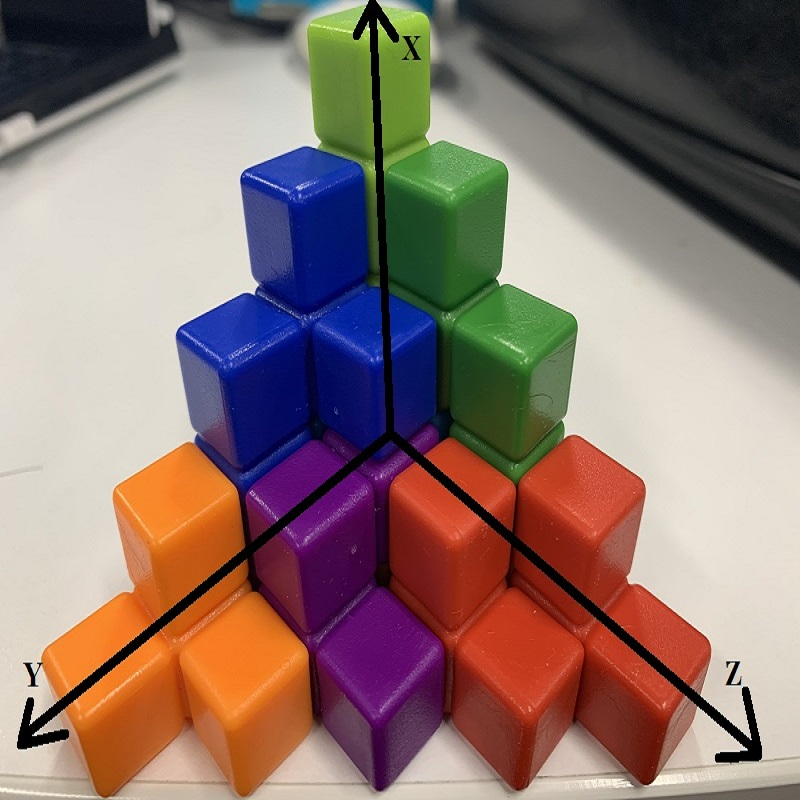
\includegraphics[width=\textwidth]{figs/3Dboard1.jpg}
\caption{}
\label{figure:mode1B}
\end{subfigure}
\caption{The board of ZIA ZAG Puzzler mode1}
  \label{fig:board1}
\end{figure}
\\For playing mode1, as is shown in Figure~\ref{fig:board1}, the maximum number for each axis is 5, hence,
\begin{equation}
\begin{aligned}
&0<x_{0}\leq5,\\
&0<y_{0}\leq5,\\
&0<z_{0}\leq5.
\end{aligned}
\end{equation}
If it is located in one of the 3 plane. Such as xy-plane $(x_{0},y_{0},1)$, it will satisfy
\begin{equation}
x_{0}+y_{0}\leq6.
\end{equation}
Accordingly, it will satisfy 
\begin{equation}
x_{0}+z_{0}\leq6
\end{equation}
in xz-plane and 
\begin{equation}
y_{0}+z_{0}\leq6
\end{equation}
in yz-plane. In addition, Figure~\ref{figure:mode1B} shows that all the units that are not in the 3 planes are close to one of the three planes, which means it's a unit of distance to one of the three plane. So we get
\begin{equation}
x_{0}+y_{0}+z_{0}\leq7.
\end{equation}
Because what we discussed above has included all positions, the domain of playing mode1 is
\begin{equation}
\begin{aligned}
&\forall \hspace{1ex} v \in \VUnits,\\
&D(v)=\{(x,y,z) \in \mathbb{Z} \times \mathbb{Z}	\times \mathbb{Z} \mid  0<x \leq 5, \hspace{1ex} 0<y \leq 5,\hspace{1ex} 0<z \leq 5,\\ &x+y\leq 6,\hspace{1ex} y+z\leq 6,\hspace{1ex}x+z\leq 6,\hspace{1ex}x+y+z\leq 7\}.
\end{aligned}
\end{equation}
\begin{figure}[htbp]
\centering
\begin{subfigure}[b]{.3\textwidth}
\centering
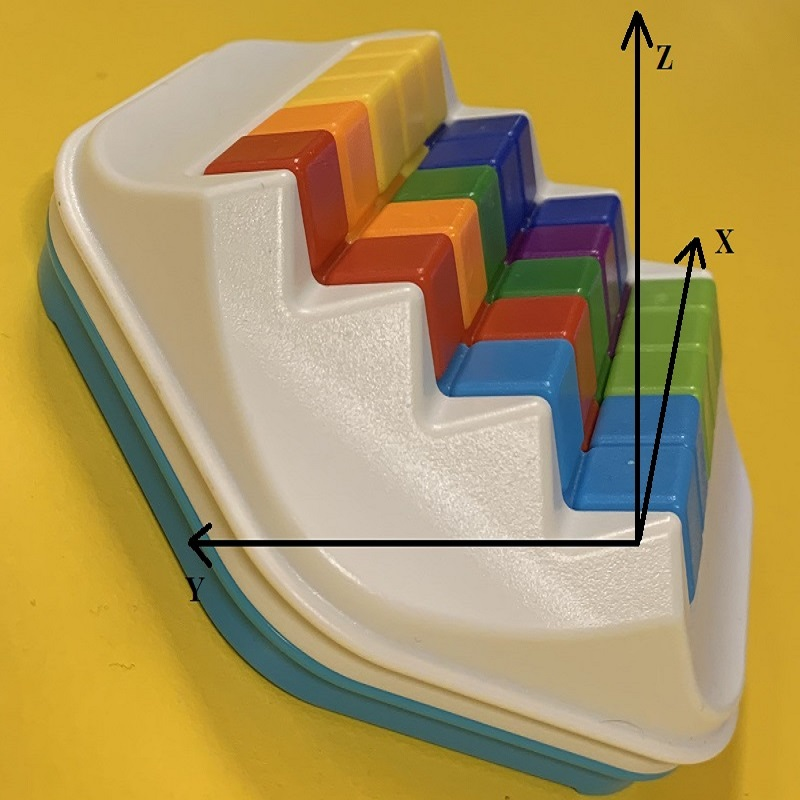
\includegraphics[width=\textwidth]{figs/ZIGZAGmodel2board.jpg}
\caption{}
\label{fig:board2A}
\end{subfigure}
\begin{subfigure}[b]{.3\textwidth}
\centering
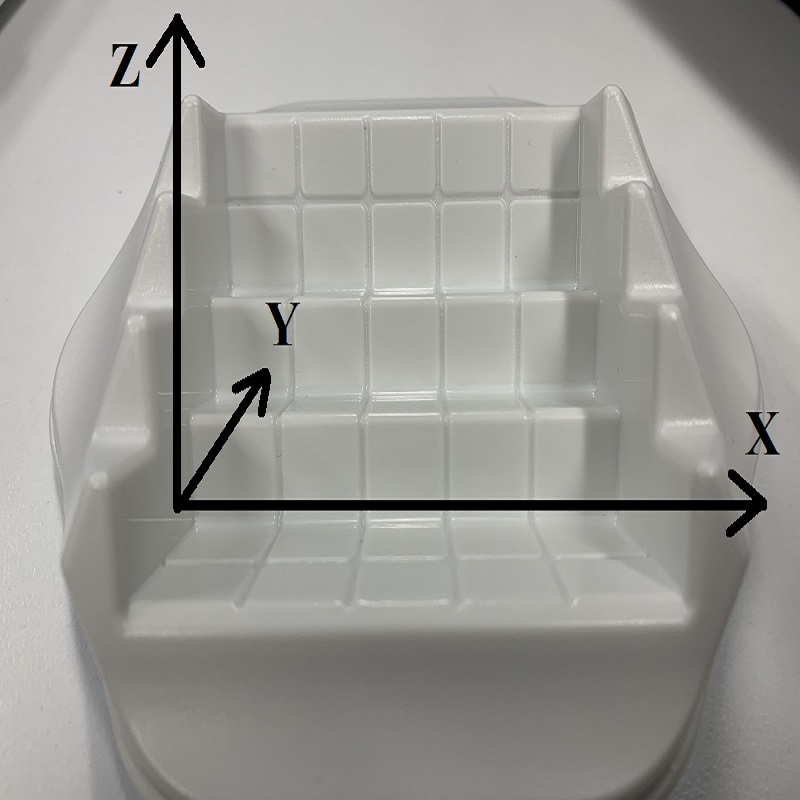
\includegraphics[width=\textwidth]{figs/3Dboard2.jpg}
\caption{}
\label{fig:board2B}
\end{subfigure}
\caption{The boards of ZIA ZAG Puzzler mode2}
  \label{fig:board2}
\end{figure}
For playing mode2, Figure~\ref{fig:board2} shows that the max number for both y-axis and z-axis are 4 and x-axis is 5, which can be represented as 
\begin{equation}
\begin{aligned}
&0<x_{0}\leq5,\\
&0<y_{0}\leq4,\\
&0<z_{0}\leq4.
\end{aligned}
\end{equation}
In addition, the board is similar to stairs, so we can get
\begin{equation}
y_{0}=z_{0}.
\end{equation}
Besides the part that is similar to stairs, the left space satisfy 
\begin{equation}
y_{0}=z_{0}+1,
\end{equation}
except when $z_{0}=4$.
Therefore, the domain of playing mode2 is
\begin{equation}
\begin{aligned}
&\forall v \in \VUnits,\\
&D(v)=\{(x,y,z) \in \mathbb{Z} \times \mathbb{Z}	\times \mathbb{Z} \mid  0<x \leq 5 , \hspace{1ex} 0<y \leq 4,\hspace{1ex} 0<z \leq 4,y=z\} \hspace{1ex}\cup\\
&\{(x,y,z) \in \mathbb{Z} \times \mathbb{Z}	\times \mathbb{Z} \mid  0<x \leq 5, \hspace{1ex} 0<y \leq 4,\hspace{1ex} 0<z \leq 3,y=z+1\}.
\end{aligned}
\end{equation}
\subsection{3D Rotation Matrix}
\label{section:3Drotationmatrix}
To clarify how to obtain all configurations for each piece.  I’d like to introduce 3D rotation matrix.
\begin{figure}[htbp]
\label{figure:3Dblue1}
\centering
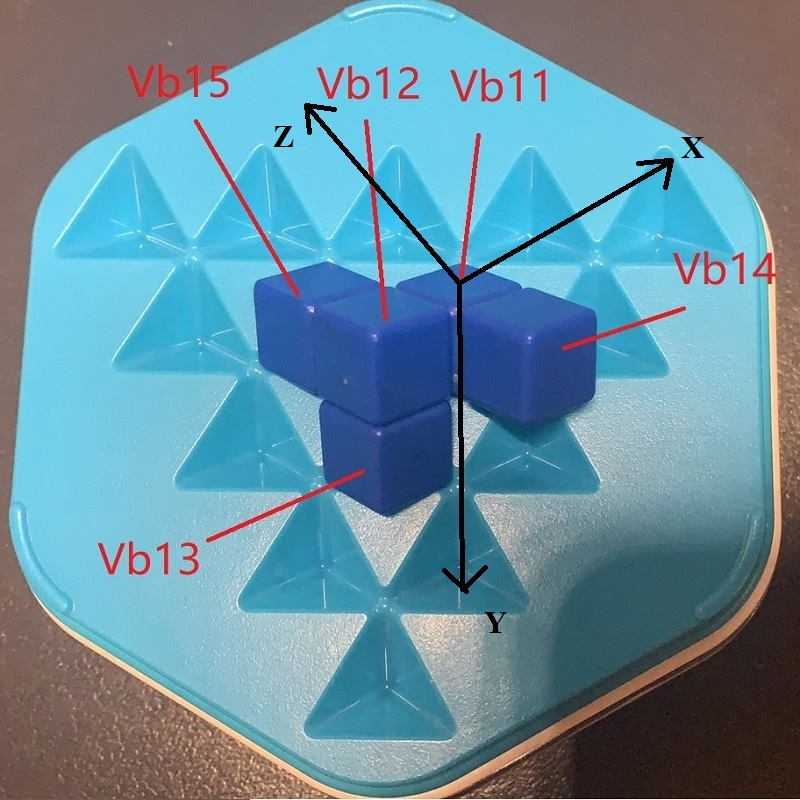
\includegraphics[width=0.3\textwidth]{figs/3Drotateexplain.jpg}
\caption{3Dblue1 initial state}
\label{fig:3Dblue1explanation}
\end{figure}
\\As is shown in Figure~\ref{fig:3Dblue1explanation}, the unit which is corresponding to the first variable $V_{b11}$ will be considered as a point $(x_{0},y_{0},z_{0})$. If we assign $(0,0,0)$ to $(x_{0},y_{0},z_{0})$, the $V_{b11}$, $V_{b12}$, $V_{b13}$, $V_{b14}$ and $V_{b15}$ are respectively represented as $(0,0,0)$, $(-1,0,0)$, $(-1,1,0)$, $(0,0,-1)$ and $(-1,0,1)$, which indicate that all other variables are connection with the first variables. For example, there are relationships
\begin{equation}
\begin{aligned}
&x_{V_{b11}}-1=x_{V_{b12}},\\
&y_{V_{b11}}=y_{V_{b12}},\\
&z_{V_{b11}}=z_{V_{b12}},
\end{aligned}
\end{equation}
between $V_{b11}$ and $V_{b12}$.
Similar to the pieces of IQ Twist, the basic idea for the pieces Zig Zag puzzler is all other units of pieces rotate around the first unit of the pieces.
\\Tobias and Krantz \cite{r9} indicate that 3D rotations can be separately represented by rotation around x-axis, y-axis, and z-axis 
\begin{equation}
\label{equation:3Dmatrix1}
\begin{aligned}
R_{x}(\theta_{1})=\begin{bmatrix}
1&          0&          0\\
0&\cos\theta_{1} & -\sin\theta_{1}\\
0&\sin\theta_{1} & \cos\theta_{1}\\
\end{bmatrix},
\\R_{y}(\theta_{2})=\begin{bmatrix}
  \cos\theta_{2}&          0&\sin\theta_{2}\\
           0&          1& 0\\
-\sin\theta_{2} &          0&\cos\theta_{2}\\
\end{bmatrix},
\\R_{z}(\theta_{3})=\begin{bmatrix}
\cos\theta_{3}&-\sin\theta_{3}&0\\
\sin\theta_{3}& \cos\theta_{3}&0\\
         0&          0&1\\
\end{bmatrix},
\end{aligned}
\end{equation}
where $R_{x}(\theta_{1})$ is corresponding to rotation around x-axis by $\theta_{1}$, $R_{y}(\theta_{2})$ is corresponding to the rotation around y-axis by $\theta_{2}$ and $R_{z}(\theta_{3})$ is corresponding to the rotation around z-axis by $\theta_{3}$. In addition, if a point rotate around x-axis by $\alpha$, y-axis by $\theta$ and z-axis by $\gamma$ at the same time, the combination of the three matrix in Equation~\ref{equation:3Dmatrix1} can be represented as
\begin{equation}
\label{equation:3Dmatrix2}
\begin{aligned}
&R=R_{z}(\alpha)R_{y}(\beta)R_{x}(\gamma)=\\
&\begin{bmatrix}
\cos\alpha\cos\beta&\cos\alpha\sin\beta\sin\gamma-\sin\alpha\cos\gamma&\cos\alpha\sin\beta\cos\gamma+\sin\alpha\sin\gamma\\
\sin\alpha\cos\beta&\sin\alpha\sin\beta\sin\gamma+\cos\alpha\cos\gamma&\sin\alpha\sin\beta\cos\gamma-\cos\alpha\sin\gamma\\
         -\sin\beta&                               \cos\beta\sin\gamma&\cos\beta\cos\gamma\\
\end{bmatrix}.
\end{aligned}
\end{equation}
In our case, we only consider 0, 90, 180 and 270 degrees rotations for each axis. If we separately consider each axis, there should be four configurations for each. As an example, according to $R_{x}(\theta_{1})$ in Equation~\ref{equation:3Dmatrix1}, when the point(x,y,z) rotate around x-axis by $\theta_{1}$, we get
\begin{equation}
\begin{bmatrix}
x'\\
y'\\
z'\\
\end{bmatrix}
=R_{x}(\theta_{1})
\begin{bmatrix}
x\\
y\\
z\\
\end{bmatrix}
\end{equation}, which implies
\begin{equation}
\label{equation:theta1}
\begin{aligned}
&x'=x,\\
&y'=y\cos\theta_{1}-z\sin\theta_{1},\\
&z'=y\sin\theta_{1}+z\cos\theta_{1}.
\end{aligned}
\end{equation}
Therefore, if we assign $0^{\circ}, 90^{\circ}, 180^{\circ}, 270^{\circ}$ to $\theta_{1}$ in Equation~\ref{equation:theta1}, we obtain $(x,y,z)$, $(x,-z,y)$, $(x,-y,-z)$ and $(x,z,-y)$.
Similarly, if a point rotates around the y-axis and the z-axis by $0^{\circ}$, $90^{\circ}$, $180^{\circ}$ and $270^{\circ}$, we can get 4 configurations each. Intuitively, the number of all possible configurations should be 64 because a point can rotate around x-axis by $\theta_{1}$ which is $0^{\circ}$, $90^{\circ}$, $180^{\circ}$ or $270^{\circ}$, rotate around y-axis by $\theta_{2}$ which is $0^{\circ}$, $90^{\circ}$, $180^{\circ}$ or $270^{\circ}$, and rotate around z-axis by $\theta_{3}$ which is $0^{\circ}$, $90^{\circ}$, $180^{\circ}$ or $270^{\circ}$. Therefore, the all possible situations should be the combination of $\theta_{1}$, $\theta_{2}$ and $\theta_{3}$, there should be a total of 64 configurations ($4\times 4 \times 4$). \\However, there are only 24 configurations because of the "singularities" of Euler angles set. Euler angles are three angles that used to represent the direction of rigid body in 3D space~\cite{r24}, which corresponds $\alpha$, $\beta$ and $\gamma$ in Equation~\ref{equation:3Dmatrix2}. Hughes~\cite{r19} highlights that "any set of Euler angles where the second rotation aligns the axes of the first and third rotations causes a singularity". The second rotation axis is y-axis, and the corresponding rotation angles is $\beta$. In addition, the geometric singularities only appear when $\beta=\pm90^{\circ}$ which is called "a repeated
axis sequence" as well as $\beta=0^{\circ}$ or $180^{\circ}$ which is called non-repeated axis
sequences~\cite{r17,r19}. How they cause singularities? Firstly, let us consider $\beta=\pm90^{\circ}$. If $\beta=90^{\circ}$, we get 
\begin{equation}
R_{\beta=90}=R_{z}(\alpha)R_{y}(90^{\circ})R_{x}(\gamma)=
\begin{bmatrix}
0&-\sin(\alpha-\gamma)&\cos(\alpha-\gamma)\\
0&\cos(\alpha-\gamma)&\sin(\alpha-\gamma)\\
         -1&                              0&0\\
\end{bmatrix}.
\end{equation}
And when $\beta=-90^{\circ}$, it can be seen as $\beta=270^{\circ}$ because of the periodicity, we can get 
\begin{equation}
R_{\beta=270}=R_{z}(\alpha)R_{y}(270^{\circ})R_{x}(\gamma)=
\begin{bmatrix}
0&-\sin(\alpha+\gamma)&-\cos(\alpha+\gamma)\\
0&\cos(\alpha+\gamma)&-\sin(\alpha+\gamma)\\
1&                               0&0
\end{bmatrix}.
\end{equation}
Based on the formula
\begin{equation}
\begin{bmatrix}
x'\\
y'\\
z'\\
\end{bmatrix}
=R
\begin{bmatrix}
x\\
y\\
z\\
\end{bmatrix},
\end{equation}
for $\beta=90^{\circ}$,
\begin{equation}
\label{equation:beta=90}
\begin{aligned}
&x'=-y\sin(\alpha-\gamma)-z\cos(\alpha-\gamma), \\
&y'=y\cos(\alpha-\gamma)+z\sin(\alpha-\gamma), \\
&z'=-x. 
\end{aligned}
\end{equation}
and for $\beta=270^{\circ}$, 
\begin{equation}
\label{equation:beta=270}
\begin{aligned}
&x'=-y\sin(\alpha+\gamma)-z\cos(\alpha+\gamma), \\
&y'=y\cos(\alpha+\gamma)-z\sin(\alpha+\gamma), \\
&z'=x.
\end{aligned}
\end{equation}
Because in our case, the domains of both $\alpha$ and $\gamma$ are $0^{\circ}$, $90^{\circ}$, $180^{\circ}$, $270^{\circ}$ and the period of the trigonometric function is $360^{\circ}$. For Equation~\ref{equation:beta=90}, the 4 configurations are $\alpha-\gamma$=$0^{\circ}$ or $90^{\circ}$ or $180^{\circ}$ or $270^{\circ}$. For Equation~\ref{equation:beta=270}, the 4 configurations are $\alpha+\gamma$=$0^{\circ}$ or $90^{\circ}$ or $180^{\circ}$ or $270^{\circ}$.
Therefore, these 2 groups of formulas represent that there are only 4 configurations for each of them. In other words, the separated $\alpha$ and $\gamma$ are meaningless. What we should consider is $\alpha-\gamma$ in Equation~\ref{equation:beta=90} and $\alpha+\gamma$ in Equation~\ref{equation:beta=270}. 
\\In Equation~\ref{equation:beta=90}, we assign 0,90,180 and 270 degrees to the $(\alpha-\gamma)$, we get four configurations:
\begin{itemize}
  \item  $x'=-y\sin(0^{\circ})-z\cos(0^{\circ}),\hspace{5pt} y'=y\cos(0^{\circ})+z\sin(0^{\circ}),\hspace{5pt} z'=-x \\\implies x'=-z,\hspace{5pt} y'=y,\hspace{5pt} z'=-x$
  \item  $x'=-y\sin(90^{\circ})-z\cos(90^{\circ}), \hspace{5pt} y'=y\cos(90^{\circ})+z\sin(90^{\circ}), \hspace{5pt} z'=-x\\\implies x'=-y,\hspace{5pt} y'=z,\hspace{5pt} z'=-x$
  \item  $x'=-y\sin(180^{\circ})-z\cos(180^{\circ}), \hspace{5pt} y'=y\cos(180^{\circ})+z\sin(180^{\circ}), \hspace{5pt} z'=-x\\\implies x'=z,\hspace{5pt} y'=-y,\hspace{5pt} z'=-x$
  \item  $x'=-y\sin(270^{\circ})-z\cos(270^{\circ}), \hspace{5pt} y'=y\cos(270^{\circ})+z\sin(270^{\circ}), \hspace{5pt} z'=-x\\\implies x'=y, \hspace{5pt}y'=-z,\hspace{5pt} z'=-x$
  \label{3Drotation24situations1}
\end{itemize}
In Equation~\ref{equation:beta=270}, we assign 0,90,180 and 270 degrees to the $(\alpha+\gamma)$, we get four configurations:
\begin{itemize}
  \item  $x'=-y\sin(0^{\circ})-z\cos(0^{\circ}),\hspace{5pt} y'=y\cos(0^{\circ})-z\sin(0^{\circ}),\hspace{5pt} z'=-x \\\implies x'=-z,\hspace{5pt} y'=y,\hspace{5pt} z'=x$
  \item  $x'=-y\sin(90^{\circ})-z\cos(90^{\circ}),\hspace{5pt} y'=y\cos(90^{\circ})-z\sin(90^{\circ}),\hspace{5pt} z'=-x\\\implies x'=-y,\hspace{5pt} y'=-z,\hspace{5pt} z'=x$
  \item  $x'=-y\sin(180^{\circ})-z\cos(180^{\circ}),\hspace{5pt} y'=y\cos(180^{\circ})-z\sin(180^{\circ}),\hspace{5pt} z'=-x\\\implies x'=z,\hspace{5pt} y'=-y,\hspace{5pt} z'=x$
  \item  $x'=-y\sin(270^{\circ})-z\cos(270^{\circ}),\hspace{5pt} y'=y\cos(270^{\circ})-z\sin(270^{\circ}),\hspace{5pt} z'=-x\\\implies x'=y, \hspace{5pt}y'=z,\hspace{5pt} z'=x$
  \label{3Drotation24situations2}
\end{itemize}
Then, we consider  $\beta=0^{\circ}$ and $\beta=180^{\circ}$. Based on (3.6), when $\beta=0^{\circ}$, we get
\begin{equation}
\label{equation:beta=0}
R=R_{z}(\alpha)R_{y}(0^{\circ})R_{x}(\gamma)=
\begin{bmatrix}
\cos\alpha&-\sin\alpha\cos\gamma&\sin\alpha\sin\gamma\\
\sin\alpha&\cos\alpha\cos\gamma&-\cos\alpha\sin\gamma\\
0&          \sin\gamma&\cos\gamma\\
\end{bmatrix}.
\end{equation}
When $\beta=180^{\circ}$, we get
\begin{equation}
\label{equation:beta=180}
R=R_{z}(\alpha)R_{y}(180^{\circ})R_{x}(\gamma)=
\begin{bmatrix}
-\cos\alpha&-\sin\alpha\cos\gamma&\sin\alpha\sin\gamma\\
-\sin\alpha&\cos\alpha\cos\gamma&-\cos\alpha\sin\gamma\\
0&                               -\sin\gamma&-\cos\gamma\\
\end{bmatrix}.
\end{equation}
In Equation~\ref{equation:beta=0}, we assign $\alpha=\alpha+180^{\circ}$ and $\gamma=\gamma+180^{\circ}$, then it change to
\begin{equation}
\label{equation:alphaandgamma}
\begin{aligned}
&R=R_{z}(\alpha+180^{\circ})R_{y}(180^{\circ})R_{x}(\gamma+180^{\circ})=\\
&\begin{bmatrix}
-\cos(\alpha+180^{\circ})&-\sin(\alpha+180^{\circ})\cos(\gamma+180^{\circ})&\sin(\alpha+180^{\circ})\sin(\gamma+180^{\circ})\\
-\sin(\alpha+180^{\circ})&\cos(\alpha+180^{\circ})\cos(\gamma+180^{\circ})&-\cos(\alpha+180^{\circ})\sin(\gamma+180^{\circ})\\
0&                               -\sin(\gamma+180^{\circ})&-\cos(\gamma+180^{\circ})
\end{bmatrix}\\
&=\begin{bmatrix}
\cos(\alpha)&-\sin(\alpha)\cos(\gamma)&\sin(\alpha)\sin(\gamma)\\
\sin(\alpha)&\cos(\alpha)\cos(\gamma)&-\cos(\alpha)\sin(\gamma)\\
0&                               \sin(\gamma)&\cos(\gamma)\\
\end{bmatrix}.
\end{aligned}
\end{equation}
Therefore, based on Equation~\ref{equation:beta=0} and Equation~\ref{equation:alphaandgamma},
\begin{equation}
R_{z}(\alpha)R_{y}(0^{\circ})R_{x}(\gamma)=R_{z}(\alpha+180^{\circ})R_{y}(180^{\circ})R_{x}(\gamma+180^{\circ}),
\end{equation}
which means that when $\beta=0^{\circ}$, regardless of the number of degrees of $\alpha$ and the number of degrees of $\gamma$, there are always corresponding $\alpha+180^{\circ}$, $\gamma+180^{\circ}$ when $\beta=180^{\circ}$. Even though the number of degrees of $\alpha+180^{\circ}$ or $\gamma+180^{\circ}$ may be more than $360^{\circ}$, it can always find a corresponding from $0^{\circ}$ to $360^{\circ}$ according to the periodicity of trigonometric function. For example, \begin{equation}
\begin{aligned}
&\circled{1}R_{z}(270^{\circ})Ry(0^{\circ})R_{x}(270^{\circ}) = R_{z}(450^{\circ})R_{y}(180^{\circ})R_{x}(450^{\circ})\\ 
&\circled{2}R_{z}(450^{\circ})Ry(180^{\circ})R_{x}(450^{\circ}) = R_{z}(90^{\circ})R_{y}(180^{\circ})R_{x}(90^{\circ})\\
&\circled{1},\circled{2}\implies R_{z}(270^{\circ})Ry(0^{\circ})R_{x}(270^{\circ})   = R_{z}(90^{\circ})R_{y}(180^{\circ})R_{x}(90^{\circ}).
\end{aligned}
\end{equation}
Hence, all combinations among $\beta=0^{\circ}$, $\theta=0^{\circ}$ or $90^{\circ}$ or $180^{\circ}$ or $270^{\circ}$ and $\gamma=0^{\circ}$ or $90^{\circ}$ or $180^{\circ}$ or $270^{\circ}$ can be obtained from one combination among $\beta=180^{\circ}$, $\theta=0^{\circ}$ or $90^{\circ}$ or $180^{\circ}$ or $270^{\circ}$ and $\gamma=0^{\circ}$ or $90^{\circ}$ or $180^{\circ}$ or $270^{\circ}$. So we only need to consider the all configurations when $\beta=0^{\circ}$ because the all configurations in $\beta=180^{\circ}$ are duplicates. For Equation~\ref{equation:beta=0}, we assign $\theta=0^{\circ},\gamma=0^{\circ}$; $\theta=0^{\circ},\gamma=90^{\circ}$;...;$\theta=270^{\circ},\gamma=180^{\circ}$; $\theta=270^{\circ},\gamma=270^{\circ}$. we get
\begin{itemize}
  \item  $x'=x$,   $y'=y$,    $z'=z$,
  \item  $x'=x$,   $y'=-z$,   $z'=y$, 
  \item  $x'=x$,   $y'=-y$,   $z'=-z$, 
  \item  $x'=x$,   $y'=z$,    $z'=-y$,
  \item  $x'=-y$,  $y'=x$,    $z'=z$,
  \item  $x'=z$,   $y'=x$,    $z'=y$,
  \item  $x'=y$,   $y'=x$,    $z'=-z$,
  \item  $x'=-z$,  $y'=x$,    $z'=-y$,
  \item  $x'=-x$,  $y'=-y$,   $z'=z$,
  \item  $x'=-x$,  $y'=z$,    $z'=y$,
  \item  $x'=-x$,  $y'=y$,    $z'=-z$,
  \item  $x'=-x$,  $y'=-z$,   $z'=-y$,
  \item  $x'=y$,   $y'=-x$,   $z'=z$,
  \item  $x'=-z$,  $y'=-x$,   $z'=y$,
  \item  $x'=-y$,  $y'=-x$,   $z'=-z$,
  \item  $x'=z$,   $y'=-x$,   $z'=-y$.
  \label{3Drotation24situations3}
\end{itemize}
There should be a total of 16 configurations (4$\times$4). Finally, consider the all configurations in $\beta=90^{\circ}$, $\beta=270^{\circ}$, $\beta=^{\circ}0$ and $\beta=180^{\circ}$. There should be a total of 4+4+16=24 configurations.
Therefore, if we assign $(0,0,0)$ to $Vb11$ in Figure~\ref{fig:3Dblue1explanation}, accordingly, we can get the initial state for $Vb12$, $Vb13$, $Vb14$ and $Vb15$, which corresponds as (-1,0,0), (-1,-1,0), (0,0,-1) and (-1,0,1). Based on the initial state, if all other units of piece rotate around Vb11, there should be 24 configurations. In our case, the piece can be moved as long as all units of piece on the board. Hence, on the condition of all units of piece on the board, we can assign variables $(x_{0},y_{0},z_{0})$ to $Vb11$, accordingly, we can get other units of piece's positions. Therefore, the constrains can be represented by the relationships between each other units of piece with the first unit of piece $Vb11$.
\subsection{Constraints}
According to chapter~\ref{section:3Drotationmatrix}, there are 24 rotation configurations. So we get
\begin{align*}
&\Cons{b11}{b12}{b13}{b14}{b15}=\{((x_{1},y_{1},z_{1}),(x_{2},y_{2},z_{2}),(x_{3},y_{3},z_{3}),(x_{4},y_{4},z_{4}),(x_{5},y_{5},z_{5}))\in \\
&\Domain {b11} \times \Domain{b12}\times \Domain{b13}\times \Domain{b14}\times \Domain{b15} \mid\\
&(x_{2}=x_{1}-1,\hspace{1ex} y_{2}=y_{1},\hspace{1ex} z_{2}=z_{1},\hspace{1ex} x_{3}=x_{1}-1,\hspace{1ex} y_{3}=y_{1}+1,\hspace{1ex} z_{3}=z_{1},\hspace{1ex} x_{4}=x_{1},\\
&\hspace{1ex} y_{4}=y_{1},\hspace{1ex} z_{4}=z_{1}-1,\hspace{1ex} x_{5}=x_{1}-1,\hspace{1ex} y_{5}=y_{1},\hspace{1ex} z_{5}=z_{1}+1)&or\\ 
&(x_{2}=x_{1},\hspace{1ex} y_{2}=y_{1}+1,\hspace{1ex} z_{2}=z_{1},\hspace{1ex} x_{3}=x_{1},\hspace{1ex} y_{3}=y_{1}+1,\hspace{1ex} z_{3}=z_{1}-1,\hspace{1ex} x_{4}=x_{1}-1,\\
&\hspace{1ex} y_{4}=y_{1},\hspace{1ex} z_{4}=z_{1},\hspace{1ex} x_{5}=x_{1}+1,\hspace{1ex} y_{5}=y_{1}+1,\hspace{1ex} z_{5}=z_{1})&or\\ 
&(x_{2}=x_{1},\hspace{1ex} y_{2}=y_{1}+1,\hspace{1ex} z_{2}=z_{1},\hspace{1ex} x_{3}=x_{1},\hspace{1ex} y_{3}=y_{1}+1,\hspace{1ex} z_{3}=z_{1}+1,\hspace{1ex} x_{4}=x_{1}+1,\\
&\hspace{1ex} y_{4}=y_{1},\hspace{1ex} z_{4}=z_{1},\hspace{1ex} x_{5}=x_{1}-1,\hspace{1ex} y_{5}=y_{1}+1,\hspace{1ex} z_{5}=z_{1})&or\\ 
&(x_{2}=x_{1},\hspace{1ex} y_{2}=y_{1},\hspace{1ex} z_{2}=z_{1}-1,\hspace{1ex} x_{3}=x_{1}-1,\hspace{1ex} y_{3}=y_{1},\hspace{1ex} z_{3}=z_{1}-1,\hspace{1ex} x_{4}=x_{1},\\
&\hspace{1ex} y_{4}=y_{1}+1,\hspace{1ex} z_{4}=z_{1},\hspace{1ex} x_{5}=x_{1},\hspace{1ex} y_{5}=y_{1}-1,\hspace{1ex} z_{5}=z_{1}-1)&or\\ 
&(x_{2}=x_{1}-1,\hspace{1ex} y_{2}=y_{1},\hspace{1ex} z_{2}=z_{1},\hspace{1ex} x_{3}=x_{1}-1,\hspace{1ex} y_{3}=y_{1}-1,\hspace{1ex} z_{3}=z_{1},\hspace{1ex} x_{4}=x_{1},\\
&\hspace{1ex} y_{4}=y_{1},\hspace{1ex} z_{4}=z_{1}+1,\hspace{1ex} x_{5}=x_{1}-1,\hspace{1ex} y_{5}=y_{1},\hspace{1ex} z_{5}=z_{1}-1)&or\\ 
&(x_{2}=x_{1}+1,\hspace{1ex} y_{2}=y_{1},\hspace{1ex} z_{2}=z_{1},\hspace{1ex} x_{3}=x_{1}+1,\hspace{1ex} y_{3}=y_{1}-1,\hspace{1ex} z_{3}=z_{1},\hspace{1ex} x_{4}=x_{1},\\
&\hspace{1ex} y_{4}=y_{1},\hspace{1ex} z_{4}=z_{1}-1,\hspace{1ex} x_{5}=x_{1}+1,\hspace{1ex} y_{5}=y_{1},\hspace{1ex} z_{5}=z_{1}+1)&or\\ 
&(x_{2}=x_{1},\hspace{1ex} y_{2}=y_{1}-1,\hspace{1ex} z_{2}=z_{1},\hspace{1ex} x_{3}=x_{1},\hspace{1ex} y_{3}=y_{1}-1,\hspace{1ex} z_{3}=z_{1}-1,\hspace{1ex} x_{4}=x_{1}+1,\\
&\hspace{1ex} y_{4}=y_{1},\hspace{1ex} z_{4}=z_{1},\hspace{1ex} x_{5}=x_{1}-1,\hspace{1ex} y_{5}=y_{1}-1,\hspace{1ex} z_{5}=z_{1})&or\\ 
&(x_{2}=x_{1},\hspace{1ex} y_{2}=y_{1}-1,\hspace{1ex} z_{2}=z_{1},\hspace{1ex} x_{3}=x_{1},\hspace{1ex} y_{3}=y_{1}-1,\hspace{1ex} z_{3}=z_{1}+1,\hspace{1ex} x_{4}=x_{1}-1,\\
&\hspace{1ex} y_{4}=y_{1},\hspace{1ex} z_{4}=z_{1},\hspace{1ex} x_{5}=x_{1}+1,\hspace{1ex} y_{5}=y_{1}-1,\hspace{1ex} z_{5}=z_{1})&or\\ 
&(x_{2}=x_{1},\hspace{1ex} y_{2}=y_{1}+1,\hspace{1ex} z_{2}=z_{1},\hspace{1ex} x_{3}=x_{1}+1,\hspace{1ex} y_{3}=y_{1}+1,\hspace{1ex} z_{3}=z_{1},\hspace{1ex} x_{4}=x_{1},\\
&\hspace{1ex} y_{4}=y_{1},\hspace{1ex} z_{4}=z_{1}-1,\hspace{1ex} x_{5}=x_{1},\hspace{1ex} y_{5}=y_{1}+1,\hspace{1ex} z_{5}=z_{1}+1)&or\\ 
&(x_{2}=x_{1},\hspace{1ex} y_{2}=y_{1},\hspace{1ex} z_{2}=z_{1}+1,\hspace{1ex} x_{3}=x_{1},\hspace{1ex} y_{3}=y_{1}-1,\hspace{1ex} z_{3}=z_{1}+1,\hspace{1ex} x_{4}=x_{1}+1,\\
&\hspace{1ex} y_{4}=y_{1},\hspace{1ex} z_{4}=z_{1},\hspace{1ex} x_{5}=x_{1}-1,\hspace{1ex} y_{5}=y_{1},\hspace{1ex} z_{5}=z_{1}+1)&or\\ 
&(x_{2}=x_{1},\hspace{1ex} y_{2}=y_{1},\hspace{1ex} z_{2}=z_{1}+1,\hspace{1ex} x_{3}=x_{1}+1,\hspace{1ex} y_{3}=y_{1},\hspace{1ex} z_{3}=z_{1}+1,\hspace{1ex} x_{4}=x_{1},\\
&\hspace{1ex} y_{4}=y_{1}+1,\hspace{1ex} z_{4}=z_{1},\hspace{1ex} x_{5}=x_{1},\hspace{1ex} y_{5}=y_{1}-1,\hspace{1ex} z_{5}=z_{1}+1)&or\\ 
&(x_{2}=x_{1},\hspace{1ex} y_{2}=y_{1},\hspace{1ex} z_{2}=z_{1}-1,\hspace{1ex} x_{3}=x_{1},\hspace{1ex} y_{3}=y_{1}+1,\hspace{1ex} z_{3}=z_{1}-1,\hspace{1ex} x_{4}=x_{1}+1,\\
&\hspace{1ex} y_{4}=y_{1},\hspace{1ex} z_{4}=z_{1},\hspace{1ex} x_{5}=x_{1}-1,\hspace{1ex} y_{5}=y_{1},\hspace{1ex} z_{5}=z_{1}-1)&or\\ 
&(x_{2}=x_{1},\hspace{1ex} y_{2}=y_{1}-1,\hspace{1ex} z_{2}=z_{1},\hspace{1ex} x_{3}=x_{1}-1,\hspace{1ex} y_{3}=y_{1}-1,\hspace{1ex} z_{3}=z_{1},\hspace{1ex} x_{4}=x_{1},\\
&\hspace{1ex} y_{4}=y_{1},\hspace{1ex} z_{4}=z_{1}-1,\hspace{1ex} x_{5}=x_{1},\hspace{1ex} y_{5}=y_{1}-1,\hspace{1ex} z_{5}=z_{1}+1)&or\\ 
&(x_{2}=x_{1}+1,\hspace{1ex} y_{2}=y_{1},\hspace{1ex} z_{2}=z_{1},\hspace{1ex} x_{3}=x_{1}+1,\hspace{1ex} y_{3}=y_{1},\hspace{1ex} z_{3}=z_{1}-1,\hspace{1ex} x_{4}=x_{1},\\
&\hspace{1ex} y_{4}=y_{1}+1,\hspace{1ex} z_{4}=z_{1},\hspace{1ex} x_{5}=x_{1}+1,\hspace{1ex} y_{5}=y_{1}-1,\hspace{1ex} z_{5}=z_{1})&or\\
&(x_{2}=x_{1}+1,\hspace{1ex} y_{2}=y_{1},\hspace{1ex} z_{2}=z_{1},\hspace{1ex} x_{3}=x_{1}+1,\hspace{1ex} y_{3}=y_{1}+1,\hspace{1ex} z_{3}=z_{1},\hspace{1ex} x_{4}=x_{1},\\
&\hspace{1ex} y_{4}=y_{1},\hspace{1ex} z_{4}=z_{1}+1,\hspace{1ex} x_{5}=x_{1}+1,\hspace{1ex} y_{5}=y_{1},\hspace{1ex} z_{5}=z_{1}-1)&or\\ 
&(x_{2}=x_{1},\hspace{1ex} y_{2}=y_{1},\hspace{1ex} z_{2}=z_{1}-1,\hspace{1ex} x_{3}=x_{1},\hspace{1ex} y_{3}=y_{1}-1,\hspace{1ex} z_{3}=z_{1}-1,\hspace{1ex} x_{4}=x_{1}-1,\\
&\hspace{1ex} y_{4}=y_{1},\hspace{1ex} z_{4}=z_{1},\hspace{1ex} x_{5}=x_{1}+1,\hspace{1ex} y_{5}=y_{1},\hspace{1ex} z_{5}=z_{1}-1)&or\\ 
&(x_{2}=x_{1},\hspace{1ex} y_{2}=y_{1},\hspace{1ex} z_{2}=z_{1}+1,\hspace{1ex} x_{3}=x_{1},\hspace{1ex} y_{3}=y_{1}+1,\hspace{1ex} z_{3}=z_{1}+1,\hspace{1ex} x_{4}=x_{1}-1,\\
&\hspace{1ex} y_{4}=y_{1},\hspace{1ex} z_{4}=z_{1},\hspace{1ex} x_{5}=x_{1}+1,\hspace{1ex} y_{5}=y_{1},\hspace{1ex} z_{5}=z_{1}+1)&or\\ 
&(x_{2}=x_{1},\hspace{1ex} y_{2}=y_{1},\hspace{1ex} z_{2}=z_{1}-1,\hspace{1ex} x_{3}=x_{1}+1,\hspace{1ex} y_{3}=y_{1},\hspace{1ex} z_{3}=z_{1}-1,\hspace{1ex} x_{4}=x_{1},\\
&\hspace{1ex} y_{4}=y_{1}-1,\hspace{1ex} z_{4}=z_{1},\hspace{1ex} x_{5}=x_{1},\hspace{1ex} y_{5}=y_{1}+1,\hspace{1ex} z_{5}=z_{1}-1)&or\\ 
&(x_{2}=x_{1},\hspace{1ex} y_{2}=y_{1}-1,\hspace{1ex} z_{2}=z_{1},\hspace{1ex} x_{3}=x_{1}+1,\hspace{1ex} y_{3}=y_{1}-1,\hspace{1ex} z_{3}=z_{1},\hspace{1ex} x_{4}=x_{1},\\
&\hspace{1ex} y_{4}=y_{1},\hspace{1ex} z_{4}=z_{1}+1,\hspace{1ex} x_{5}=x_{1},\hspace{1ex} y_{5}=y_{1}-1,\hspace{1ex} z_{5}=z_{1}-1)&or\\ 
&(x_{2}=x_{1},\hspace{1ex} y_{2}=y_{1}+1,\hspace{1ex} z_{2}=z_{1},\hspace{1ex} x_{3}=x_{1}-1,\hspace{1ex} y_{3}=y_{1}+1,\hspace{1ex} z_{3}=z_{1},\hspace{1ex} x_{4}=x_{1},\\
&\hspace{1ex} y_{4}=y_{1},\hspace{1ex} z_{4}=z_{1}+1,\hspace{1ex} x_{5}=x_{1},\hspace{1ex} y_{5}=y_{1}+1,\hspace{1ex} z_{5}=z_{1}-1)&or\\ 
&(x_{2}=x_{1}+1,\hspace{1ex} y_{2}=y_{1},\hspace{1ex} z_{2}=z_{1},\hspace{1ex} x_{3}=x_{1}+1,\hspace{1ex} y_{3}=y_{1},\hspace{1ex} z_{3}=z_{1}+1,\hspace{1ex} x_{4}=x_{1},\\
&\hspace{1ex} y_{4}=y_{1}-1,\hspace{1ex} z_{4}=z_{1},\hspace{1ex} x_{5}=x_{1}+1,\hspace{1ex} y_{5}=y_{1}+1,\hspace{1ex} z_{5}=z_{1})&or\\ 
&(x_{2}=x_{1}-1,\hspace{1ex} y_{2}=y_{1},\hspace{1ex} z_{2}=z_{1},\hspace{1ex} x_{3}=x_{1}-1,\hspace{1ex} y_{3}=y_{1},\hspace{1ex} z_{3}=z_{1}+1,\hspace{1ex} x_{4}=x_{1},\\
&\hspace{1ex} y_{4}=y_{1}+1,\hspace{1ex} z_{4}=z_{1},\hspace{1ex} x_{5}=x_{1}-1,\hspace{1ex} y_{5}=y_{1}-1,\hspace{1ex} z_{5}=z_{1})&or\\ 
&(x_{2}=x_{1},\hspace{1ex} y_{2}=y_{1},\hspace{1ex} z_{2}=z_{1}+1,\hspace{1ex} x_{3}=x_{1}-1,\hspace{1ex} y_{3}=y_{1},\hspace{1ex} z_{3}=z_{1}+1,\hspace{1ex} x_{4}=x_{1},\\
&\hspace{1ex} y_{4}=y_{1}-1,\hspace{1ex} z_{4}=z_{1},\hspace{1ex} x_{5}=x_{1},\hspace{1ex} y_{5}=y_{1}+1,\hspace{1ex} z_{5}=z_{1}+1)&or\\ 
&(x_{2}=x_{1}-1,\hspace{1ex} y_{2}=y_{1},\hspace{1ex} z_{2}=z_{1},\hspace{1ex} x_{3}=x_{1}-1,\hspace{1ex} y_{3}=y_{1},\hspace{1ex} z_{3}=z_{1}-1,\hspace{1ex} x_{4}=x_{1},\\
&\hspace{1ex} y_{4}=y_{1}-1,\hspace{1ex} z_{4}=z_{1},\hspace{1ex} x_{5}=x_{1}-1,\hspace{1ex} y_{5}=y_{1}+1,\hspace{1ex} z_{5}=z_{1})\}.
\end{align*}
Similarly, we can get the constraints for other pieces.
\section{Implementation}